%%%%%%%%%%%%%%%%%%%%%%%%%%%%%%%%%%%%%%%%%
% Short Sectioned Assignment LaTeX Template Version 1.0 (5/5/12)
% This template has been downloaded from: http://www.LaTeXTemplates.com
% Original author:  Frits Wenneker (http://www.howtotex.com)
% License: CC BY-NC-SA 3.0 (http://creativecommons.org/licenses/by-nc-sa/3.0/)
%%%%%%%%%%%%%%%%%%%%%%%%%%%%%%%%%%%%%%%%%

%----------------------------------------------------------------------------------------
%	PACKAGES AND OTHER DOCUMENT CONFIGURATIONS
%----------------------------------------------------------------------------------------

\documentclass[paper=a4, fontsize=11pt]{scrartcl} % A4 paper and 11pt font size

% ---- Entrada y salida de texto -----

\usepackage[T1]{fontenc} % Use 8-bit encoding that has 256 glyphs
\usepackage[utf8]{inputenc}
%\usepackage{fourier} % Use the Adobe Utopia font for the document - comment this line to return to the LaTeX default

% ---- Idioma --------

\usepackage[spanish, es-tabla]{babel} % Selecciona el español para palabras introducidas automáticamente, p.ej. "septiembre" en la fecha y especifica que se use la palabra Tabla en vez de Cuadro

% ---- Otros paquetes ----

\usepackage{amsmath,amsfonts,amsthm} % Math packages
%\usepackage{graphics,graphicx, floatrow} %para incluir imágenes y notas en las imágenes
\usepackage{graphics,graphicx, float, url} %para incluir imágenes y colocarlas

% Para hacer tablas comlejas
%\usepackage{multirow}
%\usepackage{threeparttable}
\usepackage{float}


%\usepackage{sectsty} % Allows customizing section commands
%\allsectionsfont{\centering \normalfont\scshape} % Make all sections centered, the default font and small caps

\usepackage{fancyhdr} % Custom headers and footers
\pagestyle{fancyplain} % Makes all pages in the document conform to the custom headers and footers
\fancyhead{} % No page header - if you want one, create it in the same way as the footers below
\fancyfoot[L]{} % Empty left footer
\fancyfoot[C]{} % Empty center footer
\fancyfoot[R]{\thepage} % Page numbering for right footer
\renewcommand{\headrulewidth}{0pt} % Remove header underlines
\renewcommand{\footrulewidth}{0pt} % Remove footer underlines
\setlength{\headheight}{13.6pt} % Customize the height of the header

\numberwithin{equation}{section} % Number equations within sections (i.e. 1.1, 1.2, 2.1, 2.2 instead of 1, 2, 3, 4)
\numberwithin{figure}{section} % Number figures within sections (i.e. 1.1, 1.2, 2.1, 2.2 instead of 1, 2, 3, 4)
\numberwithin{table}{section} % Number tables within sections (i.e. 1.1, 1.2, 2.1, 2.2 instead of 1, 2, 3, 4)

\setlength\parindent{0pt} % Removes all indentation from paragraphs - comment this line for an assignment with lots of text

\newcommand{\horrule}[1]{\rule{\linewidth}{#1}} % Create horizontal rule command with 1 argument of height


\title{	
	\normalfont \normalsize 
	\textsc{{\bf Ingeniería de Servidores (2014-2015)} \\ Grado en Ingeniería Informática \\ Universidad de Granada} \\ [25pt] % Your university, school and/or department name(s)
	\horrule{0.5pt} \\[0.4cm] % Thin top horizontal rule
	\huge Memoria Práctica 2 \\ % The assignment title
	\horrule{2pt} \\[0.5cm] % Thick bottom horizontal rule
}

\author{Iván Sevillano García} % Nombre y apellidos

\date{\normalsize\today} % Incluye la fecha actual

\begin{document}

\maketitle % Muestra el Título

\newpage %inserta un salto de página

\tableofcontents % para generar el índice de contenidos

\newpage

\section{Instalación de servicios y configuraciones.}
En esta sección se responden a las preguntas referentes a la administración y configuración de software en los distintos sistemas operativos.
\subsection{Yum. Gestor de paquetes de CentOS.}

Esta aplicación es el gestor predeterminado de CentOS, Red Hat, Fedora y derivados.

\begin{itemize}
	\item \textbf{Liste los argumentos de yum necesarios para instalar, buscar y eliminar paquetes.}\\
	Según el manual de yum\cite{yum}, para instalar un paquete del que ya sabemos el nombre podremos utilizar yum seguido del comando \textbf{install} tras el que pondremos el paquete a instalar. También existe la orden \textbf{groupinstall}, que instala un grupo de paquetes de forma conjunta. En realidad funciona igual que la orden install junto al nombre de todos los paquetes del grupo.\\
	
	Para buscar, el comando \textbf{search} seguido de alguna referencia indirecta del paquete(parte del nombre en general) nos dará como resultado los paquetes que tengan algo que ver con la clave de búsqueda.\\
	
	Para eliminar paquetes, yum tiene comandos \textbf{remove} y \textbf{erase} seguidos del paquete a eliminar, lo que produce redundancia de funciones, ya que hacen exactamente el mismo trabajo. Esto es un fallo de diseño y se deberá eliminar uno de estos términos en un futuro.\\
	
	\item \textbf{¿Que hay que hacer para que yum tenga acceso a internet en el aula de prácticas(puesto que esta utiliza un proxy por detrás)?}\\
	
	Para contestar a esta pregunta se nos ofrece dos pistas: acceder al archivo de configuración de yum en /etc/yum/ y que el proxy a utilizar es \textbf{stargate.ugr.es:3128}. Buscamos en el manual de configuración de yum\cite{yum.conf} y nos dice que necesitamos incluir en el archivo \textbf{yum.conf} la URL del proxy. También hay opciones para acceder al proxy con un usuario y una contraseña(proxy\_username y proxy\_password).
	
\end{itemize}

\subsection{Apt. Gestor de paquetes de Debian.}
Esta aplicación es el gestor predeterminado de Debian y sus derivados, como por ejemplo ubuntu.
\begin{itemize}
	\item \textbf{Indique el comando para buscar un paquete en un repositorio y el correspondiente para instalarlo.}\\
	Según el manual de apt\cite{apt}, para buscar un paquete del que tenemos parte del nombre o similar, debemos utilizar el comando \textbf{apt search}, y para instalarlo, el comando \textbf{apt install}.
	
	
	 \item \textbf{Indique qué ha modificado para que apt pueda acceder a los servidores de paquetes a través del proxy. ¿Cómo añadimos un nuevo repositorio?}\\
	 Según el manual proporcionado por apt.conf\cite{apt.conf}:\\
	 
	 "\textit{http::Proxy define el proxy predeterminado que utilizar para direcciones HTTP URI. Utiliza el formato estándar
	 	http://[[usuario][:contraseña]@]máquina[:puerto]/. También se puede especificar un proxy por cada máquina usando la forma
	 	http::Proxy::<máquina> con la palabra especial DIRECT que significa que no se use ningún proxy. La variable de entorno http\_proxy
	 	se usará en caso de no definir ninguna de las opciones anteriores.
	 }"\\
	 
	 También según el mismo manual, la forma de añadir repositorios es añadirlos al archivo /etc/apt/sources.list con permisos de root. Se puede utilizar el comando edit-sources, con el mismo resultado que editarlos con un editor de texto directamente, ya que este comando solo llama a un editor a escoger\cite{apt}.
	 
\end{itemize}

\subsection{Cuestión opcional: Gestor de paquetes de OpenSUSE.}
Por cuestión de tiempo, en esta asignatura no utilizaremos OpenSUSE, pero si vamos a responder a la pregunta de cuál es el gestor de paquetes de este Sistema Operativo.\\

En la página oficial de OpenSUSE\cite{yast}, se dice que éste tiene dos gestores, uno con un entorno gráfico y otro para consola. El primero es YaST y el segundo, Zypper.

\newpage
\section{Instalación del servicio de acceso seguro(SSH)}
 
 Para el acceso remoto desde una máquina a otra hay distintos protocolos. Entre ellos, destacan telnet y ssh. Sin embargo, para las conexiones que realizaremos, utilizaremos ssh. La instalación del servidor en Ubuntu se realiza con el comando:\\
 
 $sudo$ $apt$ $install$ $openssh$-$server$\\
 
 
 \begin{itemize}
 	\item ¿Cuál es la diferencia entre telnet y ssh?\\
 	Telnet\cite{telnet} es un servicio básico de conexión entre máquinas, en el cuál sólo hay envío y recepción de mensajes. Ssh\cite{ssh} (Secure shell), además de esto, los mensajes se envían de forma segura mediante distintos métodos, como pueden ser la encriptación de información. En definitiva, ssh está varios niveles por encima de telnet. Usar ssh en las prácticas es esencial ya que es mucho mas completo.
 	
 	\item ¿Para qué sirve la opción -X de ssh? Ejecute remotamente, es decir, desde la máquina anfitriona (si tiene Linux) o desde la otra máquina virtual, el comando gedit en una sesión abierta con ssh. ¿Qué ocurre?\\
 	
 	La opción -X habilita la interfaz gráfica en las sesiones ssh\cite{ssh-client}. Sin embargo, para que esto tenga sentido, la interfaz gráfica tiene que estar instalada en ambas máquinas, además de que el servidor tiene que aceptar en su archivo de configuración\cite{sshd_config} la posibilidad de utilizar la misma. Este parametro es $ForwardX11Trusted$. Veamos ahora que ocurre:\\
 	
 	Para probar esta opción, tenemos una máquina servidor y otra cliente con la interfaz gráfica de el editor de textos gedit instalada:
 	
 	\begin{figure}[H]
		\centering
		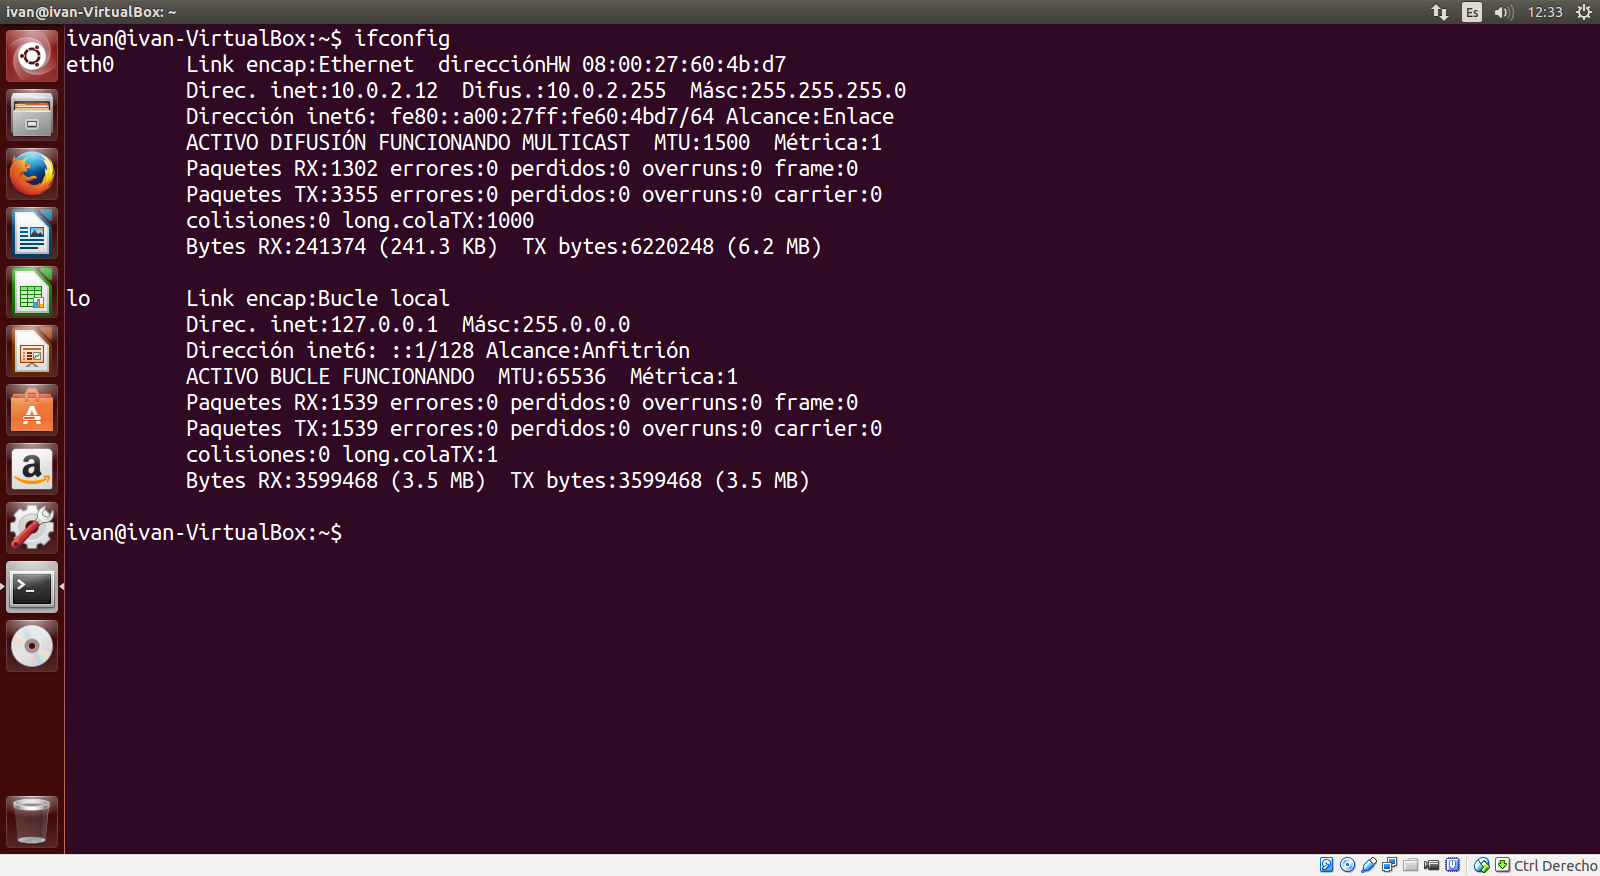
\includegraphics[width=0.7\linewidth]{clientessh-X}
		\caption[Cliente]{Máquina cliente. IP:10.0.2.12}
		\label{fig:clientessh-X}
	\end{figure}
	
	\begin{figure}[H]
		\centering
		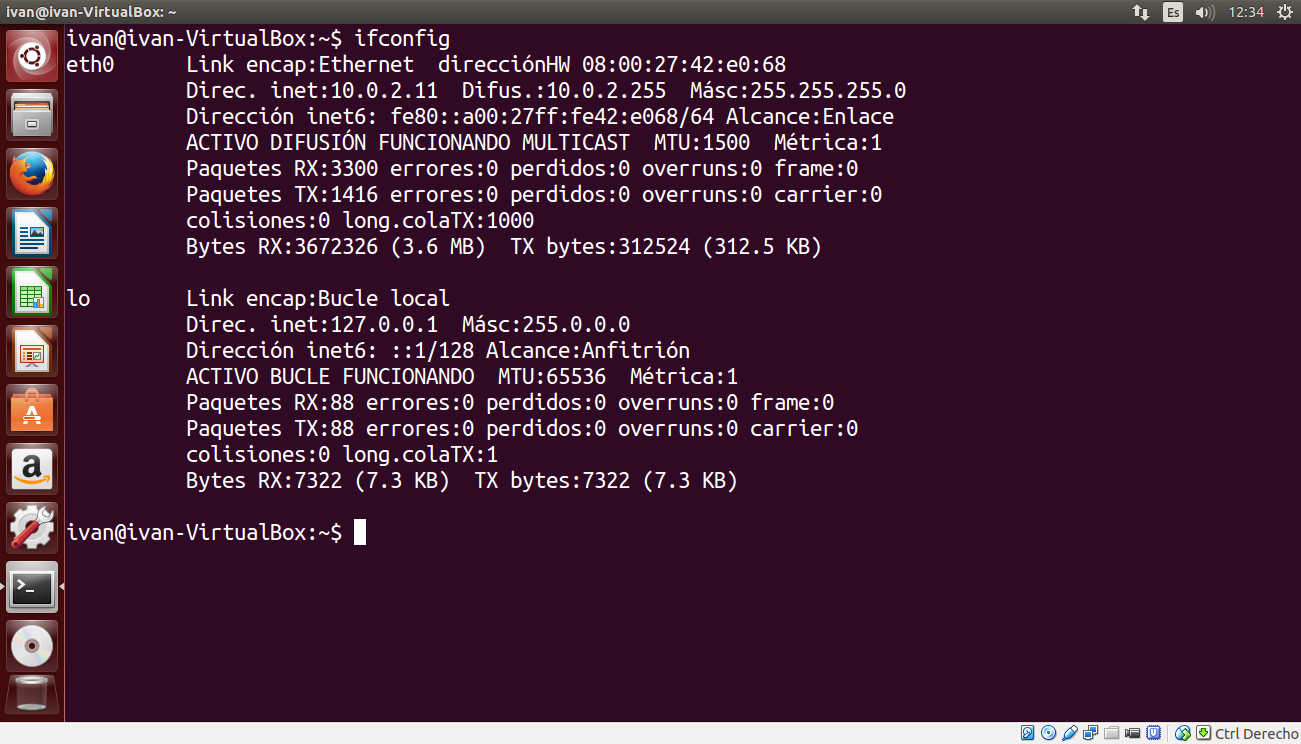
\includegraphics[width=0.7\linewidth]{servidorssh-X}
		\caption[Servidor]{Máquina servidor. IP:10.0.2.11}
		\label{fig:servidorssh-X}
	\end{figure}
	
	\begin{figure}[H]
	\centering
	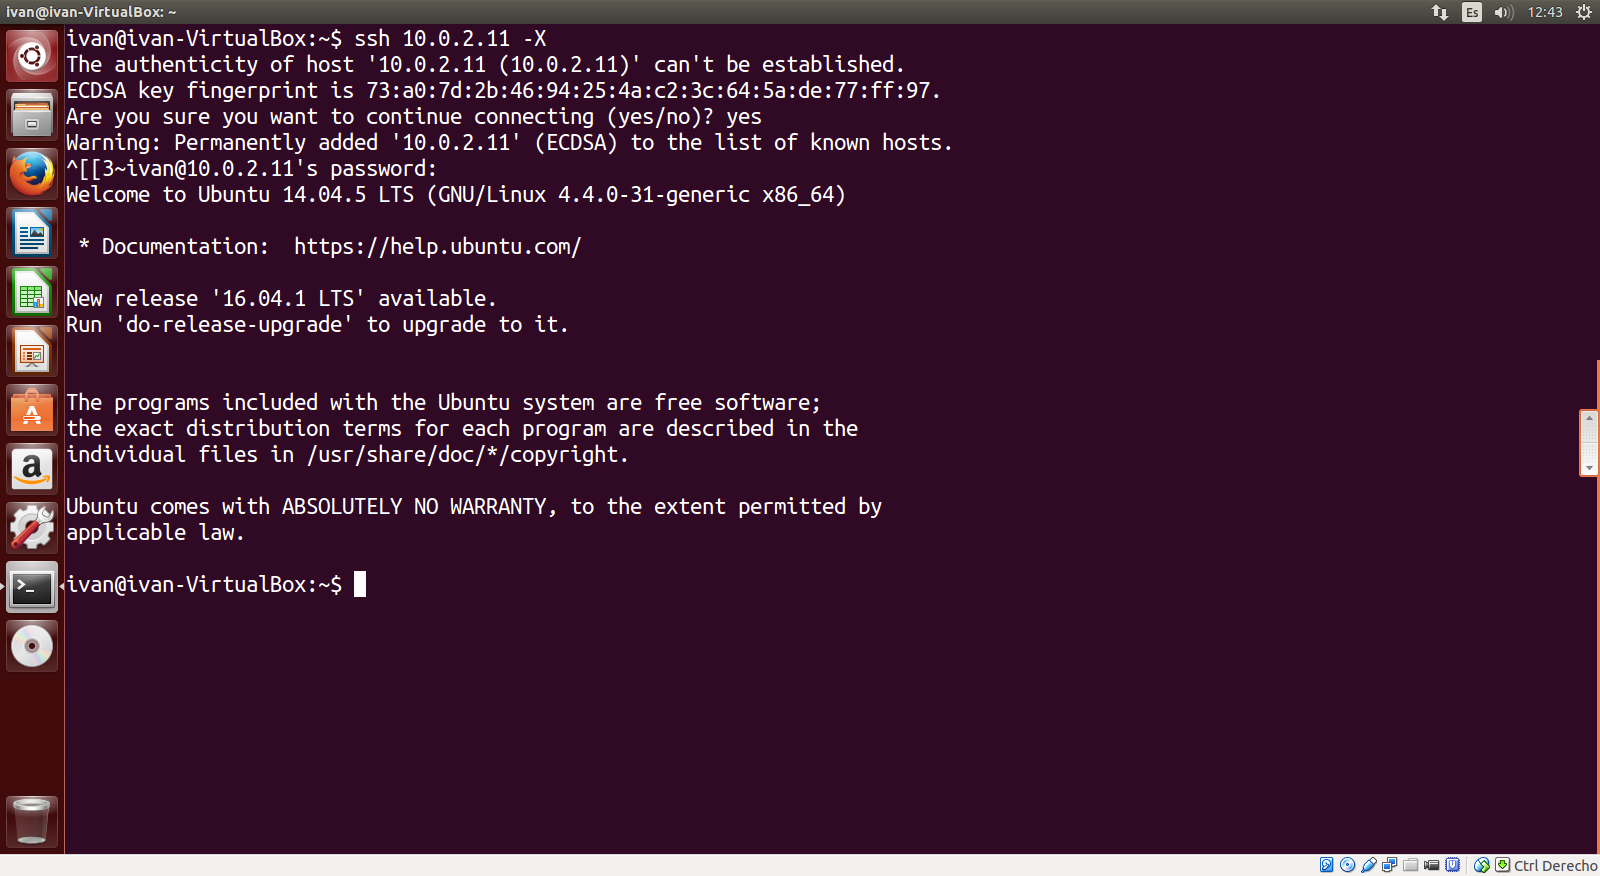
\includegraphics[width=0.7\linewidth]{Conexion-X}
	\caption[Conexión -X]{Conexión realizada con la opción -X}
	\label{fig:Conexion-X}
	\end{figure}

	
	La conexión se lleva a cabo con normalidad. Probemos ahora a utilizar gedit:
	\begin{figure}[H]
	\centering
	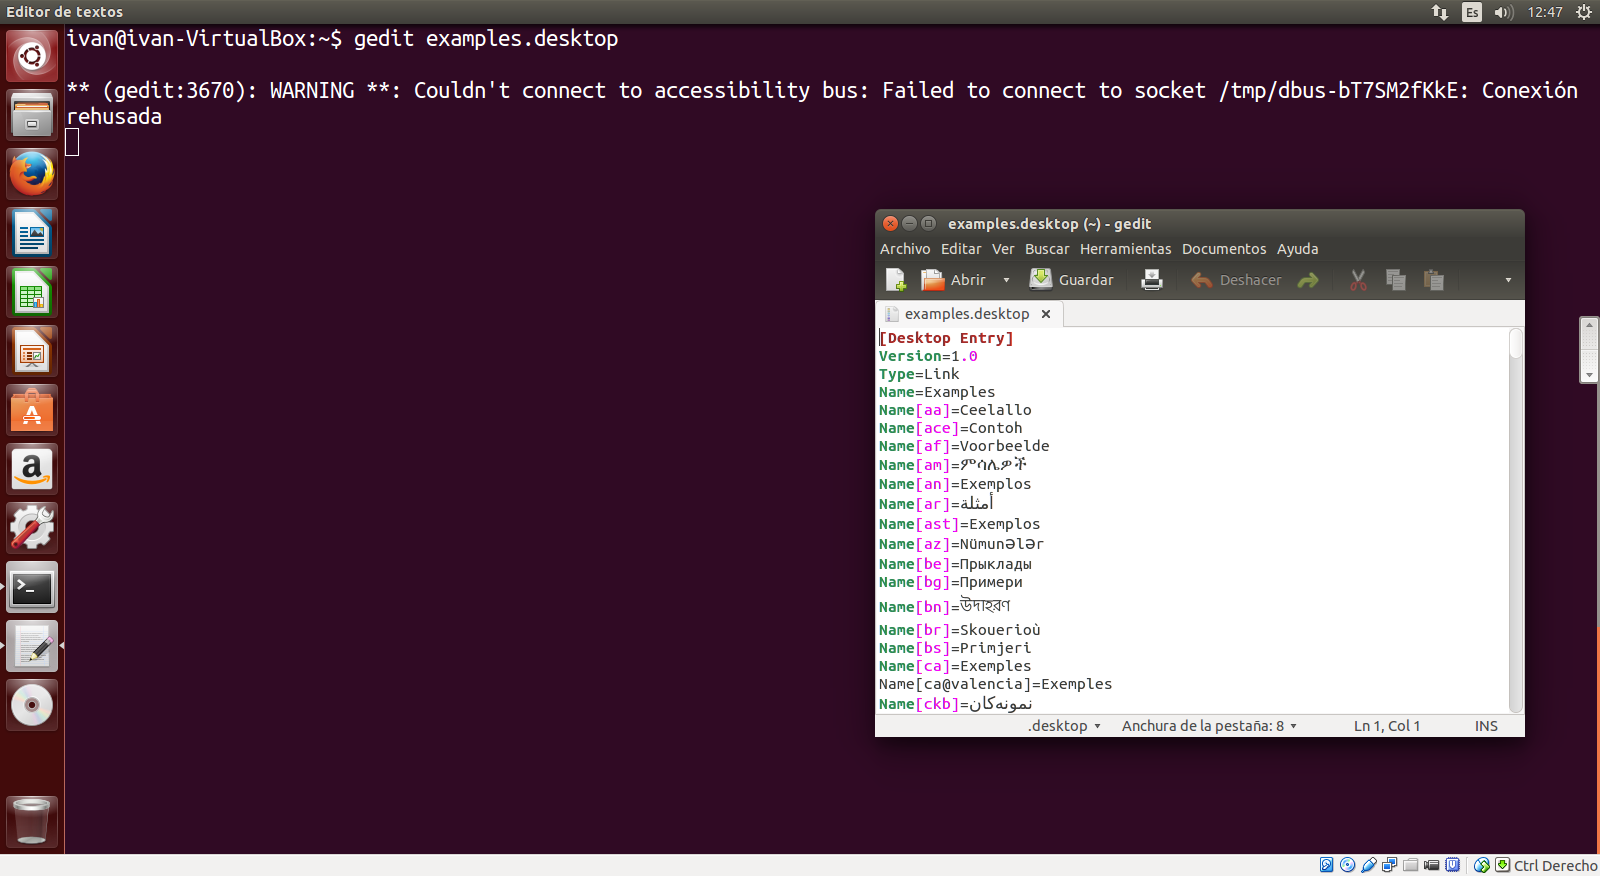
\includegraphics[width=0.7\linewidth]{UsoGedit}
	\caption[Uso Gedit]{Gedit con la opción -X}
	\label{fig:UsoGedit}
	\end{figure}
	
	Como vemos, él uso de gedit se lleva a cabo con normalidad. ¿Pero que ocurriría si utilizamos un entorno gráfico no instalado en el servidor? Cambiamos ahora a un servidor sin entorno gráfico:\\
	
	\begin{figure}[H]
	\centering
	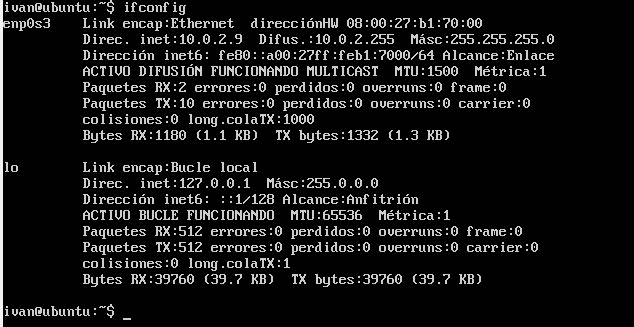
\includegraphics[width=0.7\linewidth]{servidor-no-grafico}
	\caption[Servidor no gráfico]{Máquina servidor sin entorno gráfico. IP:10.0.2.9}
	\label{fig:servidor-no-grafico}
	\end{figure}
	
	La conexión la llevamos a cabo normalmente, como se ve a continuación:\\
	
	\begin{figure}[H]
	\centering
	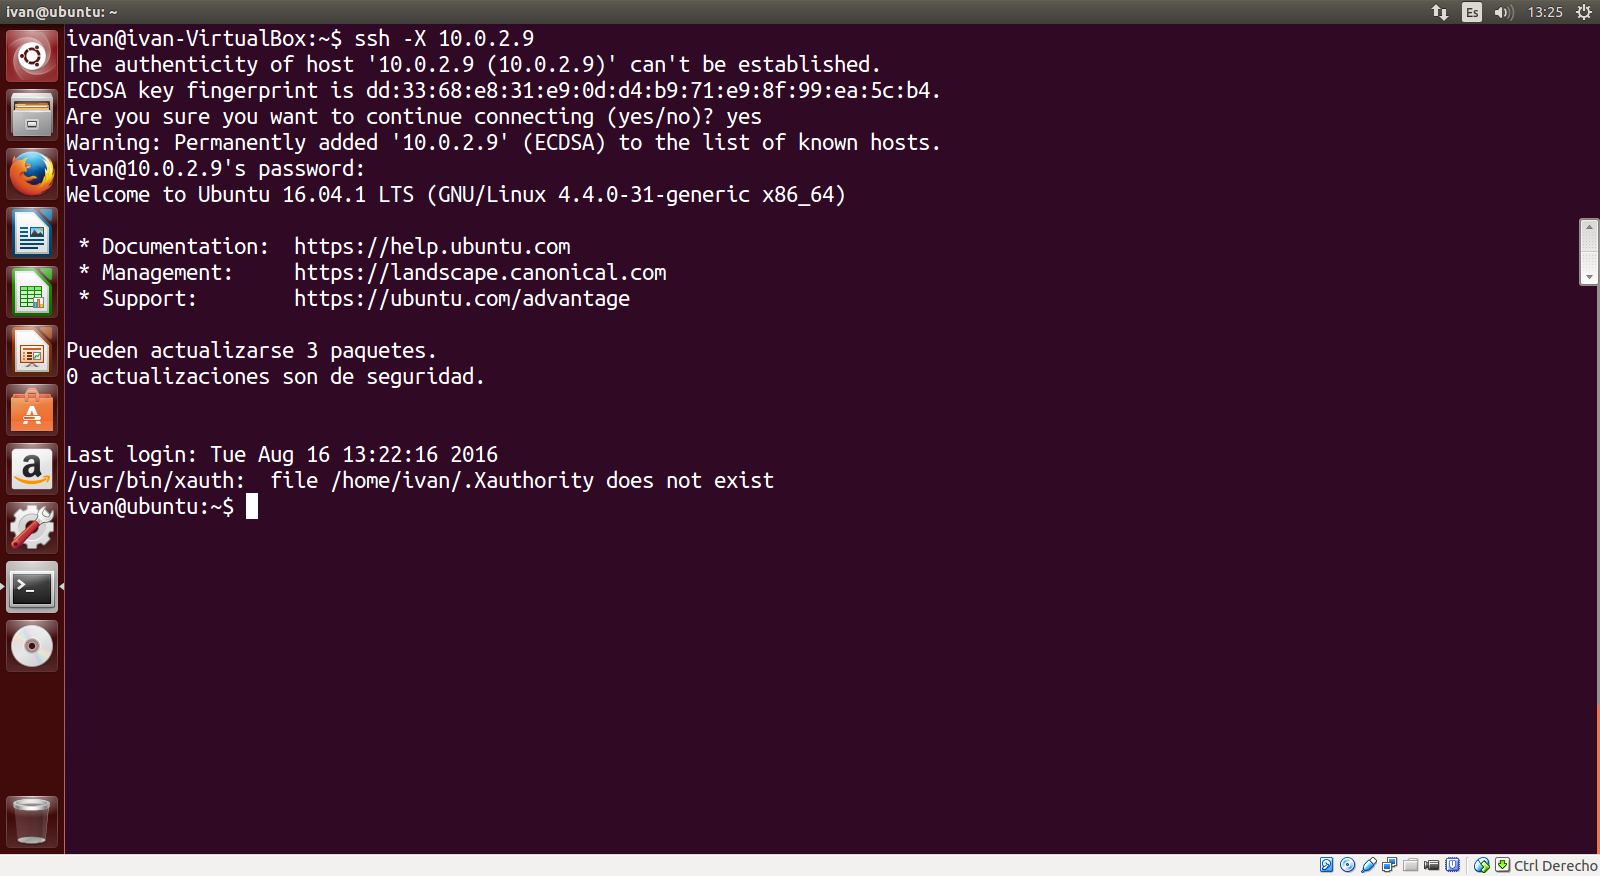
\includegraphics[width=0.7\linewidth]{Conexion-no-grafica}
	\caption[Conexión no gráfica]{Conexión con la opción -X en un servidor sin entorno gráfico.}
	\label{fig:Conexion-no-grafica}
	\end{figure}
	
	Ahora intentamos usar gedit:\\
	
	\begin{figure}[H]
	\centering
	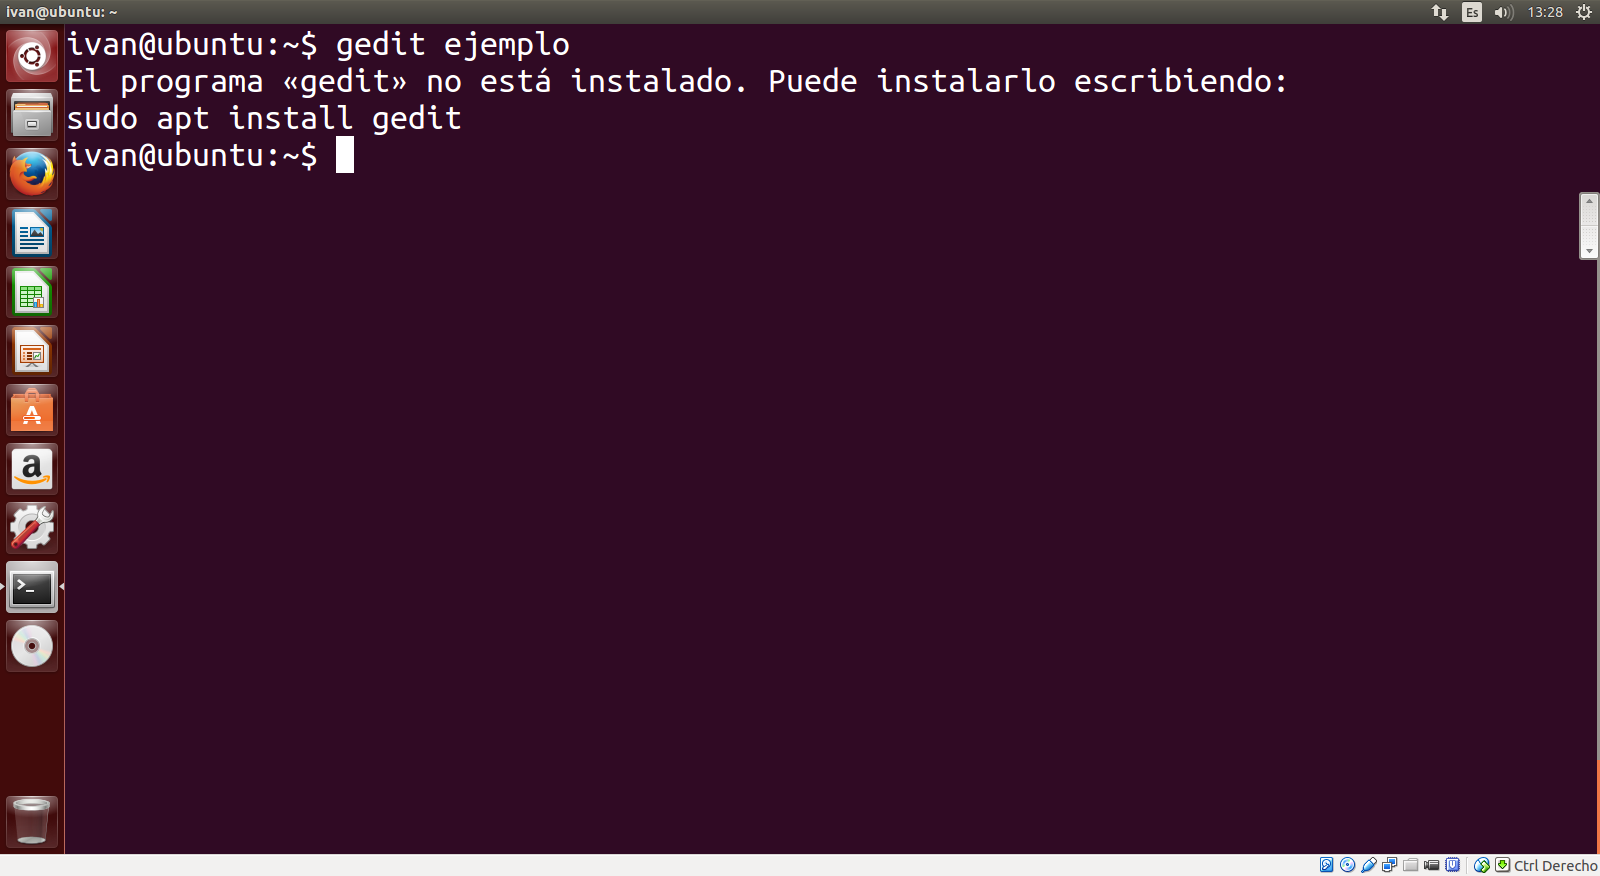
\includegraphics[width=0.7\linewidth]{gedit_fail}
	\caption[Fallo gedit]{Gedit no instalado en el servidor.}
	\label{fig:gedit_fail}
	\end{figure}
	
	Como vemos, para poder utilizar gedit, este tiene que estar instalado en el servidor. Además, este también tiene que estar instalado en el cliente.
 	
 \end{itemize}
 
 \subsection{Seguridad en ssh. Clave pública.}
 
 Tras instalar el servicio openssh-server en la máquina, probaremos ahora a conectarnos remotamente. Sin embargo, como vemos a continuación, la máquina anfitrión nos pide una contraseña(la contraseña de la cuenta):\\
 
 \begin{figure}[H]
	\centering
	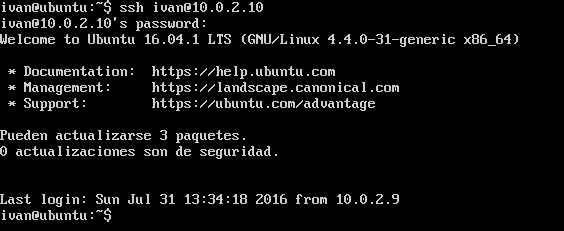
\includegraphics[width=0.7\linewidth]{ssh_no_clave}
	\caption[Sesión ssh]{Conexión ssh hecha con normalidad. Nos pide password del usuario en el servidor.}
	\label{fig:ssh_no_clave}
\end{figure}

Sin embargo, esta conexión puede ser insegura. Para hacerla más segura, vamos a utilizar el algoritmo RSA. Para ello generaremos una clave pública en el cliente que enviaremos al servidor. Con esto conseguimos que cada vez que intentemos conectarnos al servidor, no nos pregunte la contraseña de la cuenta del servidor. Esta es la secuencia de operaciones:\\

\begin{figure}[H]
	\centering
	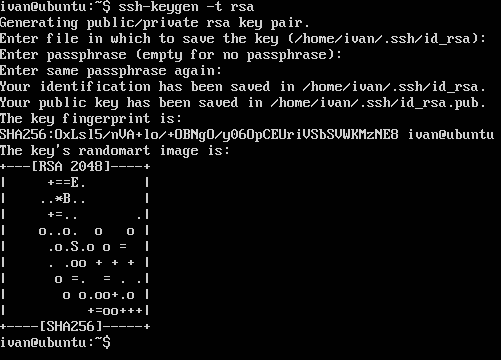
\includegraphics[width=0.7\linewidth]{keygen}
	\caption[Generando clave]{Comando ssh-keygen generando clave RSA}
	\label{fig:keygen}	
\end{figure}

En esta imagen se muestra cuales son los pasos a seguir para generar con ssh-keygen la clave. Según el manual de ssh-keygen\cite{ssh-keygen}, hay muchas opciones, pero la que nos interesa a nosotros es la opción -$t$, que especifica el protocolo que usaremos. Tras esto, keygen nos pregunta que si queremos ponerle una clave, que no será la clave pública, si no una clave interna de paso del ordenador que no pasará a la red. Nos pregunta también por donde guardar la clave. Dejaremos que la guarde por defecto en $/home/ivan/.ssh/id\_rsa.pub$. \\

El siguiente paso será enviar la clave pública al servidor para que nos identifique:

\begin{figure}[H]
	\centering
	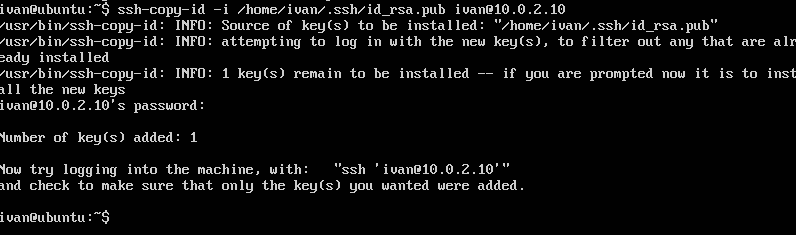
\includegraphics[width=0.7\linewidth]{ssh-copy-id}
	\caption[Uso de copy-id]{Envío de clave pública mediante ssh-copy-id}
	\label{fig:ssh-copy-id}
\end{figure}
 
Según el manual de ssh-copy-id\cite{copy-id}, la forma de uso es indicando la clave pública, con la opción -i, y el servidor ssh. Las últimas líneas de información nos dicen que ya está configurado para poder acceder a la cuenta con la clave pública. Probamos ahora a conectarnos.

\begin{figure}[H]
	\centering
	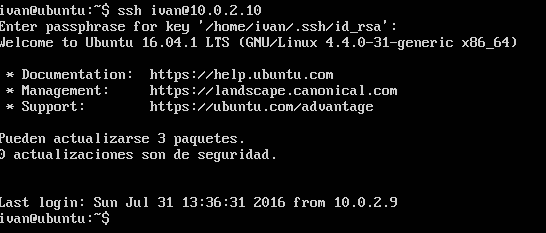
\includegraphics[width=0.7\linewidth]{ssh_con_clave_publica}
	\caption[Conexión usando clave pública]{Conexión usando la clave pública como elemento de identificación.}
	\label{fig:ssh_con_clave_publica}
\end{figure}

Como puede verse, no es necesario utilizar la contraseña de la cuenta en el servidor(La contraseña que nos pide es la generada antes internamente en el ordenador cliente para desbloquear la clave pública).
\subsection{Sshd. El demonio de ssh.}
\begin{itemize}
	\item ¿Qué archivo es el que contiene la configuración de sshd? ¿Qué parámetro hay que modificar para evitar que el usuario root acceda? Cambie el puerto por defecto y compruebe que puede acceder.\\
	
\end{itemize}

Según el manual de sshd\cite{sshd}, el directorio por defecto es $/etc/sshd/sshd_config$, y cuyas opciones de configuración se detallan en \cite{sshd_config}.\\

Para evitar que el usuario root acceda hay que modificar el parámetro $PermitRootLogin$. Según el mismo manual, para inhabilitar al usuario root hay que cambiarlo a "no".\\
	
Para cambiar el puerto de escucha hay que modificar el comando $Port$ al puerto que se desee escuchar.\\
	
Para comprobar la configuración, modificaremos el puerto de escucha al 22222 y modificaremos el parámetro dicho anteriormente:\\
	
\begin{figure}[H]
	\centering
	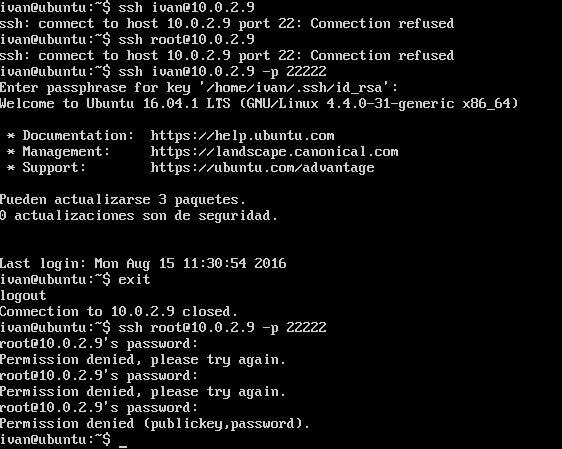
\includegraphics[width=0.7\linewidth]{conexion_puerto_22222}
	\caption[Conexión al puerto 22222]{Modificación de los parámetros Port y PermitRootLogin.}
	\label{fig:conexion_puerto_22222}
\end{figure}
	
En esta imagen se realizan cuatro intentos de conexión ssh. En los dos primeros se pide una conexión al puerto 22 por defecto, en este caso deshabilitado. La tercera conexión se realiza con el usuario ivan y se manda al puerto 22222, por lo que nos pide la contraseña interna para enviar la clave pública y nos deja conectarnos. Muy distinto es el caso en el que intentamos acceder como root, ya que aunque pongamos correcta la contraseña, no nos deja acceder.
\begin{itemize}
	\item Indique si es necesario reiniciar el servicio. ¿Cómo se reinicia un servicio en Ubuntu? ¿Y en CentOS? Muestre la secuencia de comandos para hacerlo.\\
\end{itemize}
	
Es necesario reiniciar el servicio, ya que el archivo que modificamos es un archivo de texto que tiene que ser leido por el programa antes de inicializarse. En Ubuntu, para reiniciar un servicio se utiliza $ssudo$ $service$ <$servicio$>  $start/restart$. En CentOS,$sudo$ $systemctl$ $restart$ <$servicio$>.

\subsection{Utilidades: Terminator y Screen.}

Estas dos herramientas nos sirven para abrir varios entornos de trabajo en una misma terminal. Terminator\cite{terminator} tiene distintas utilidades, como escribir en todas las terminales a la vez o asignarle distintos trabajos a las terminales dependiendo del número de ventana que sea. Para instalarlo hay que instalar el paquete terminator:\\
	
$sudo$ $apt$ $install$ $terminator$\\
	
	
\begin{figure}[H]
	\centering
	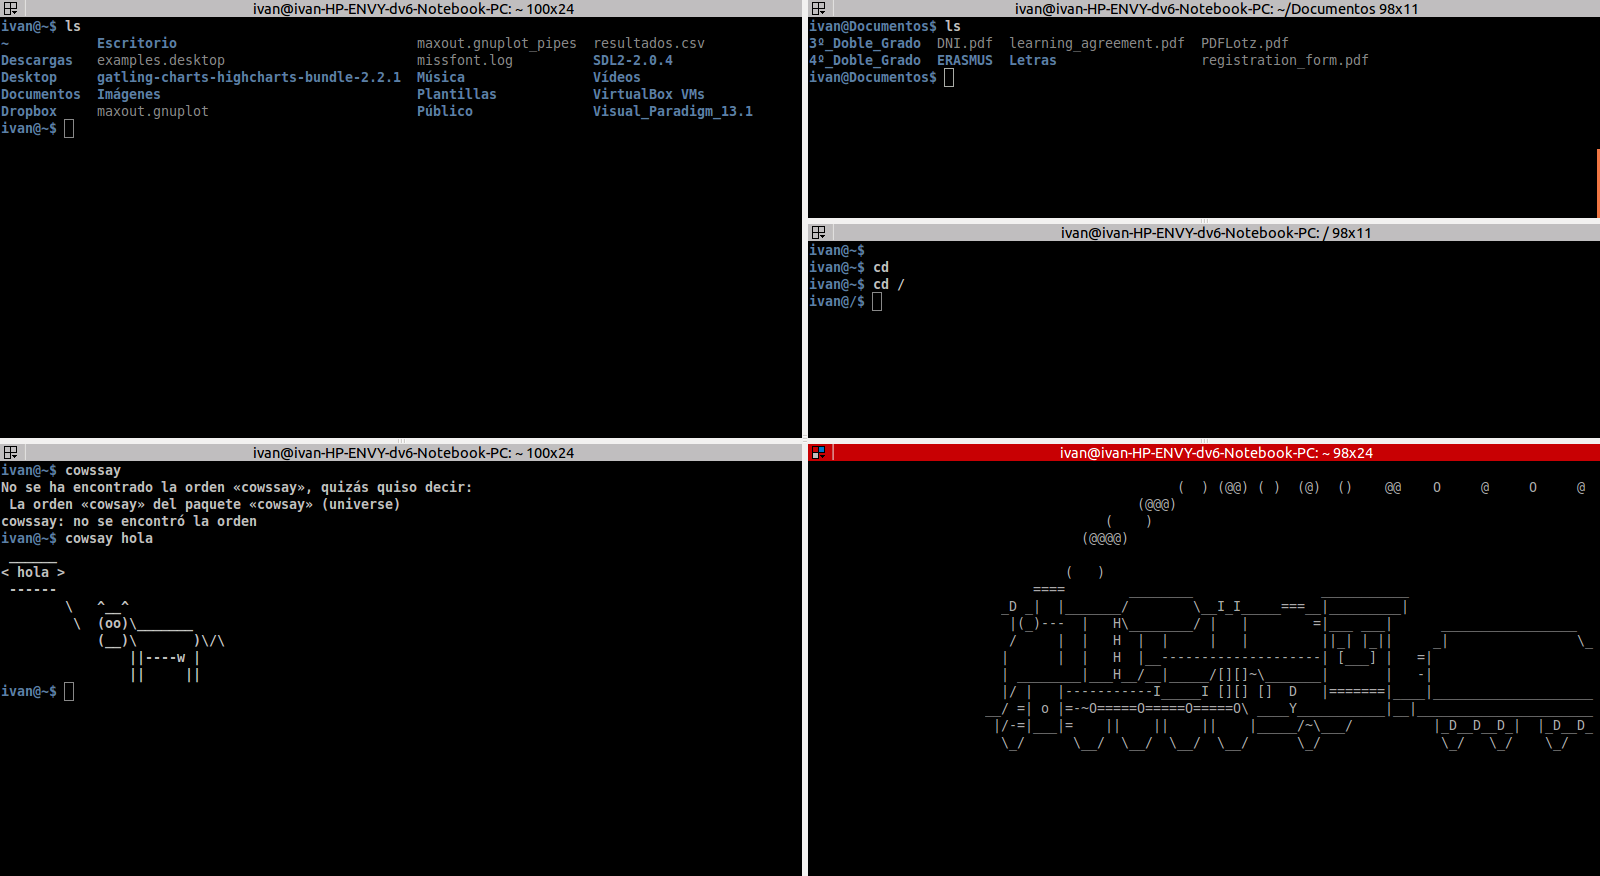
\includegraphics[width=0.7\linewidth]{terminator}
	\caption[Uso de terminator]{Ejemplo de división de ventanas con terminator.}
	\label{fig:terminator}
\end{figure}
	
La otra herramienta que se utiliza es Screen\cite{screen}. También tiene un gestor de ventanas de la terminal. Sin embargo, es más antiguo y no tiene una interfaz tan moderna como terminator. Sin embargo, puede ser usada en un servidor sin esta interfaz, ya que no le hace falta interfaz gráfica. Realizaremos ahora la conexión ssh desde screen. La dejaremos abierta para luego retomarla. \\

Al acceder a screen, primero nos aparece la siguiente salida:\\
\begin{figure}[H]
	\centering
	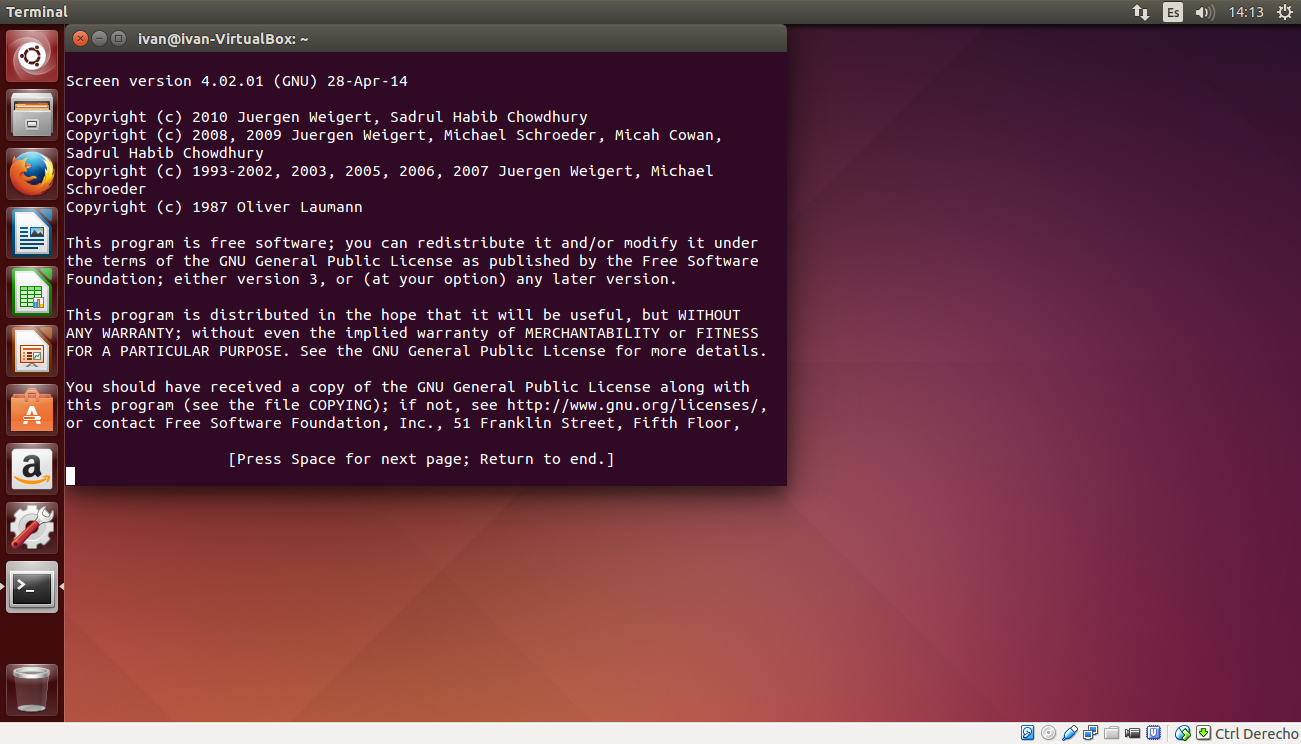
\includegraphics[width=0.7\linewidth]{ScreenConexion1}
	\caption[Screen conexión]{Salida al ejecutar screen}
	\label{fig:ScreenConexion1}
\end{figure}

tras la cual se nos abre una ventana idéntica a la de la terminal, aunque veremos que tiene mucha mas funcionalidad. Sin embargo, para ver nombrar a nuestra sesión screen y ver el proceso de forma más clara, ejecutaremos screen -S <nombre> (en nuestro caso, ivanscreen) para abrir la sesión de screen. Nos conectaremos por ssh ahora a la máquina servidora:\\

\begin{figure}[H]
	\centering
	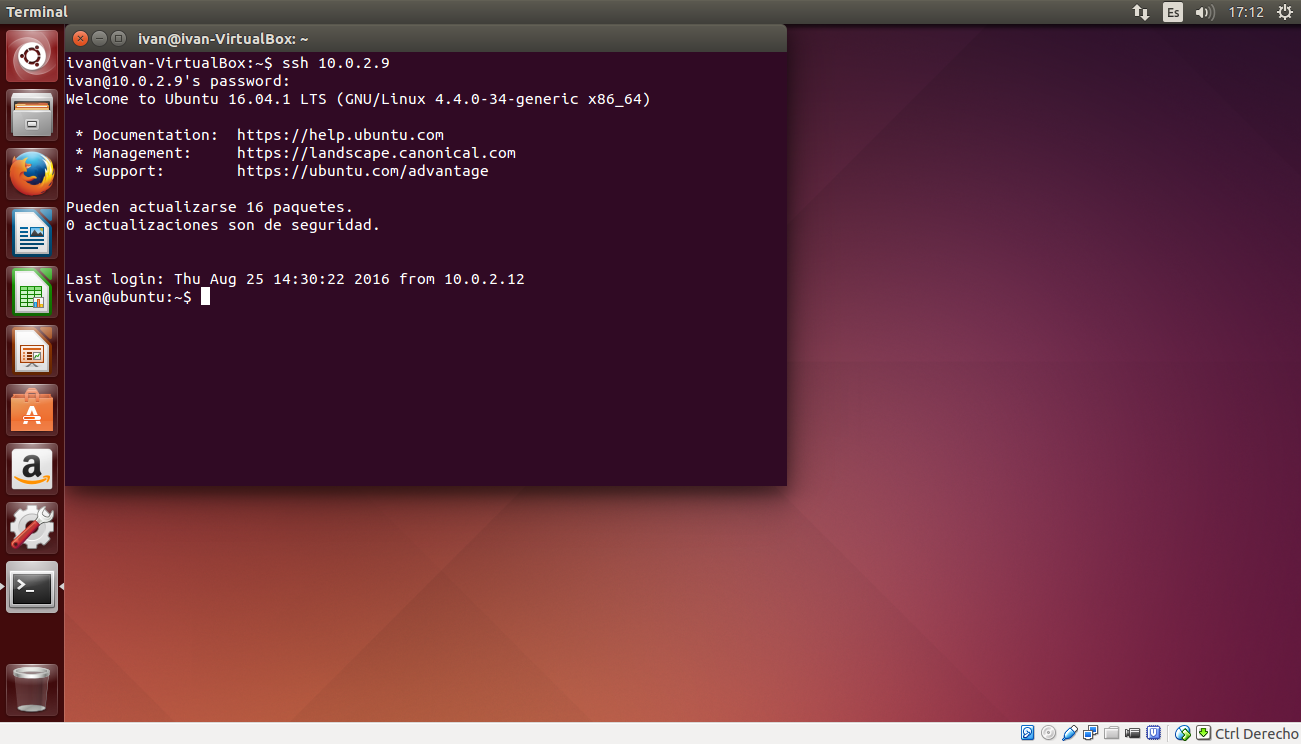
\includegraphics[width=0.7\linewidth]{screenSshNormal}
	\caption[Conexión ssh con screen]{Conexión ssh con screen}
	\label{fig:ScreenSshConection}
\end{figure}

y ahora vamos a dejarla para otro momento. Para ello, utilizaremos el comando de screen Ctrl-a d. Vemos entonces que nuestra ventana de screen ha sido $detached$. Veamos las sesiones de screen que existen en este momento(comando screen -ls):\\

\begin{figure}[H]
	\centering
	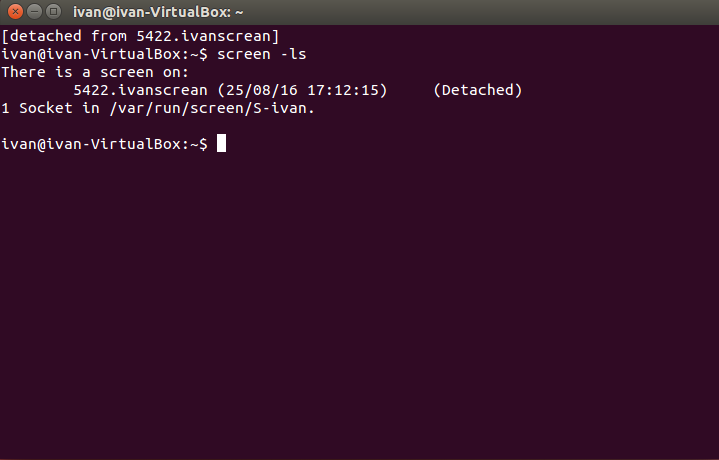
\includegraphics[width=0.7\linewidth]{ScreenDetached}
	\caption[Screen Detached]{Mensaje de screen detached y muestra de las sesiones con screen que existen.}
	\label{fig:ScreenDetached}
\end{figure}

Cabe mencionar que hemos salido de screen ya que no funcionan los atajos de teclado. Ahora, para reanudar la sesión, utilizamos el comando screen -r con el nombre de la sesión:\\

$screen$ -$r$ $ivanscreen$\\

\begin{figure}[H]
	\centering
	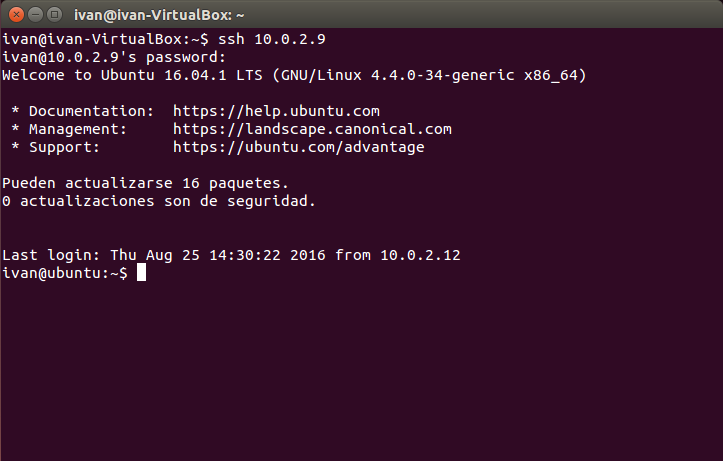
\includegraphics[width=0.7\linewidth]{ScreenVolver}
	\caption[ScreenVolver]{Sesión retomada de screen con ssh abierto.}
	\label{fig:ScreenVolver}
\end{figure}



\section{Instalación de un servidor Web básico.}

Esta sección está dedicada a la instalación de un servidor web básico en distintos sistemas operativos. En concreto, instalaremos los servicios LAMP(Apache,mysql o mariadb,PHP o python).
\subsection{Servidores de Ubuntu y CentOS.}
\begin{itemize}
	\item \textbf{Muestre los comandos que ha utilizado en Ubuntu Server y en CentOS (aunque en este último puede utilizar la GUI; en tal caso, realice capturas de pantalla).}\\
	
	En Ubuntu, basta con ejecutar la siguiente orden en la consola:\\
	
	$sudo$ $apt$ $install$ $lamp$-$server$\^\\
	
	tras lo cual solo tendremos que configurar la contraseña de mysql, como se muestra en la siguiente imagen:\\
	
	\begin{figure}[H]
	\centering
	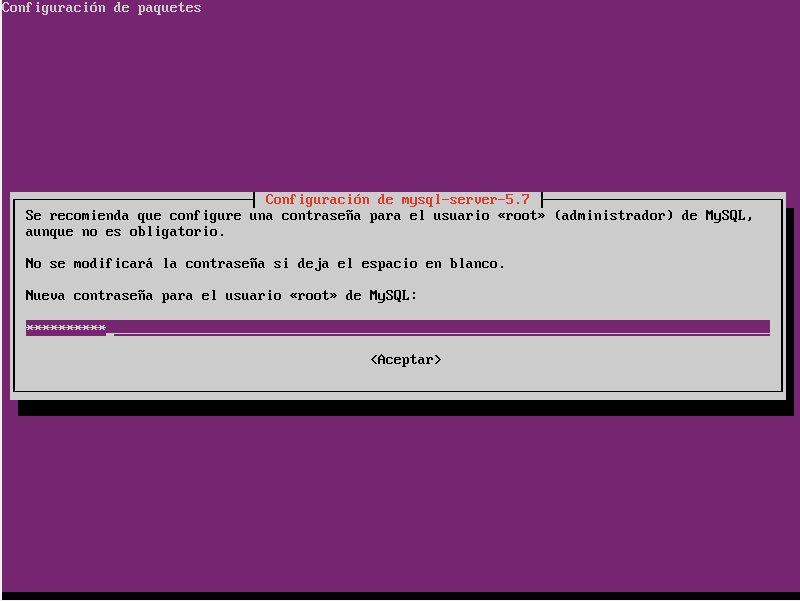
\includegraphics[width=0.7\linewidth]{Contrasena_mysql}
	\caption[Configurar contraseña]{Configurar contraseña en la instalación de mysql en Ubuntu.}
	\label{fig:Contraseña_mysql}
	\end{figure}
	
	Aquí vemos, desde otra máquina, que el servidor web está corriendo:\\
	
	\begin{figure}[H]
	\centering
	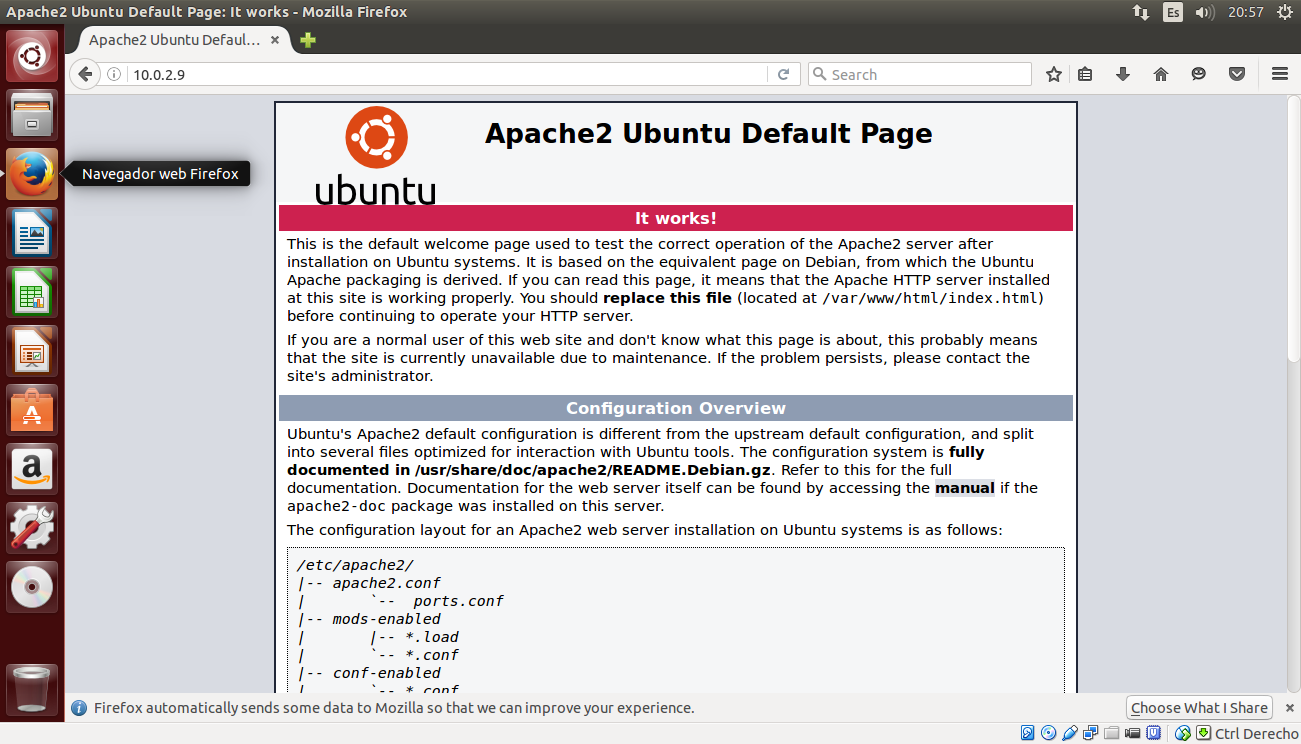
\includegraphics[width=0.7\linewidth]{Acceso_web_UbuntuServer}
	\caption[Acceso Web a Ubuntu]{Acceso a la web del servidor de Ubuntu localizado en la IP 10.0.2.9 desde una máquina con entorno gráfico.}
	\label{fig:Acceso_web_UbuntuServer}
	\end{figure}

	
	En CentOS, no existe un paquete que englobe todo lo necesario para el servidor lamp, sin embargo si se puede descargar parte a parte. Para ello, los paquetes que instalaremos serán httpd, mariadb, php y php-mysql. Con el siguiente comando, descargaremos todo:\\
	
	$sudo$ $yum$ $install$ $httpd$ $mariadb$ $php$ $php$-$mysql$
	
	A modo de confirmación, aquí dejo la salida de la terminal al introducir el comando:\\
	
	\begin{figure}[H]
	\centering
	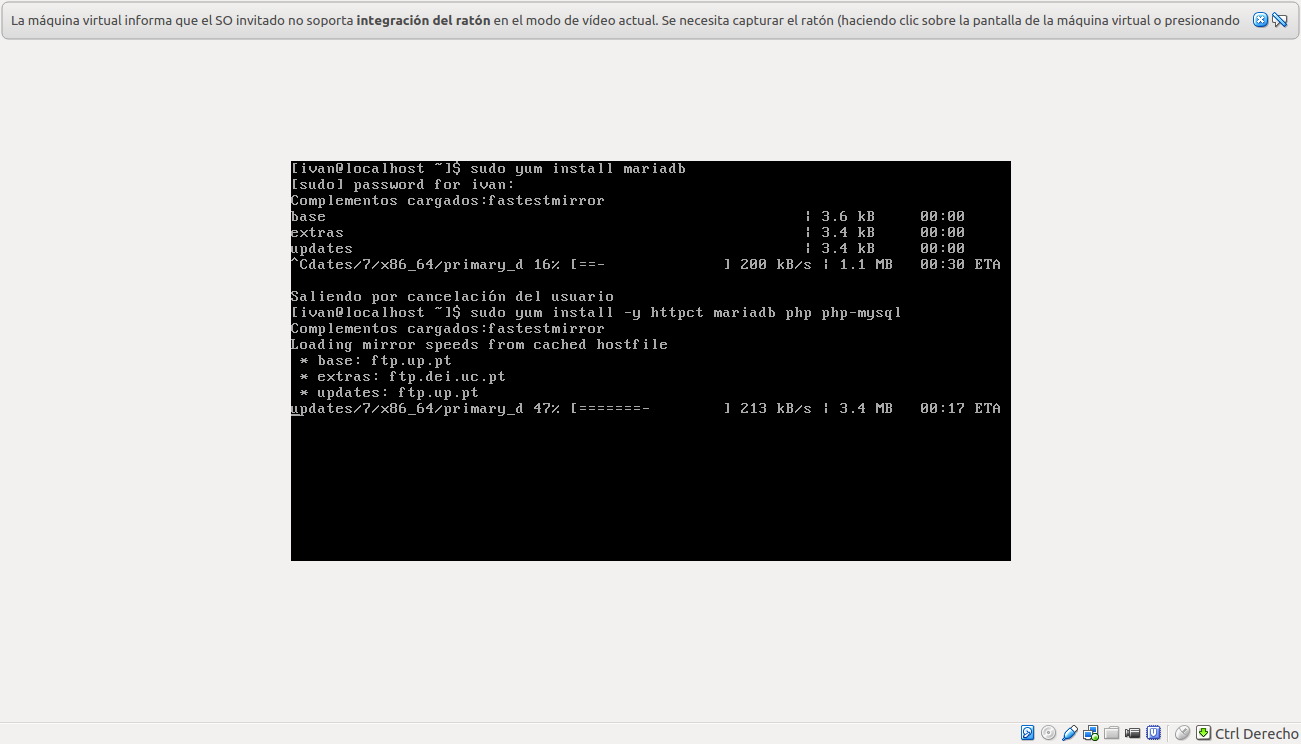
\includegraphics[width=0.7\linewidth]{instalar_lamp}
	\caption[Instalaciónlamp]{Instalación del servidor lamp en CentOS.}
	\label{fig:instalar_lamp}
	\end{figure}
	
	Al entrar desde la misma máquina con el entorno gráfico en la dirección IP del servidor CentOS, este es el resultado:\\
	
	\begin{figure}[H]
	\centering
	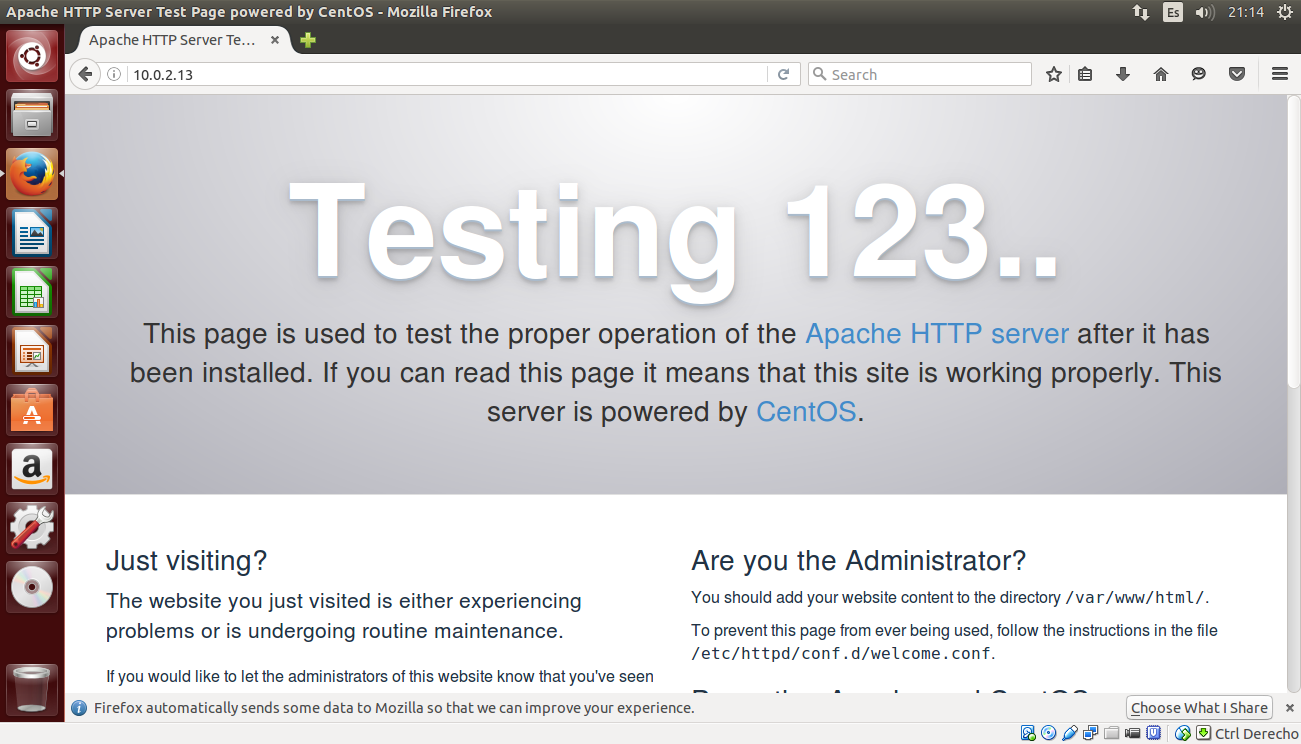
\includegraphics[width=0.7\linewidth]{AccesoWebCentos}
	\caption[AccesoWebCentos]{Acceso a la máquina que corre con CentOS localizada en la IP 10.0.2.13.}
	\caption{}
	\label{fig:Capturadepantallade2016-08-2121:14:39}
	\end{figure}

	
	En Ubuntu, para que el servidor esté completamente en orden, no hacía falta mas que la descarga del paquete. Sin embargo, en CentOS hay que poner en orden algunos puntos. Para ello tenemos que habilitar el servicio httpd, abrir los puertos del mismo y reiniciar el servicio. Por orden, estos son los comandos que hay que ejecutar:\\
	
	Habilitar el servicio web:\\
	
	$sudo$ $systemctl$ $enable$ $httpd$.$service$\\
	
	Abrir el puerto del servidor web:\\
	
	$sudo$ $firewall$-$cmd$ --$permanent$ --$add$-$service$ $http$\\
	
	Reiniciar el firewall(ya que hemos modificado los puertos que el demonio de firewall debe escuchar):\\
	
	$sudo$ $systemctl$ $restart$ $firewalld$.$service$\\
	
	
	\item \textbf{Enumere otros servidores web y las páginas de sus proyectos (mínimo 3 sin considerar Apache, IIS ni nginx)}\\
	Para contestar esta pregunta, se ha recurrido a la página oficial de w3techs\cite{w3tech}, la cual hace mediciones del número de servidores que utilizan un tipo u otro de servidor web entre otros datos(como el sistema operativo que se utiliza). Entre los servidores web que listan, se encuentran los siguientes:\\
	
	
	\begin{itemize}
		\item El proyecto LiteSpeed Web Server\cite{liteSpeed} es un proyecto de la misma compañía que vende compatibilidad con apache, mas seguridad y menos coste. 
		
		\item Apache Tomcat\cite{Tomcat} es un proyecto que desarrolla mucho software de Java. Es un proyecto de código abierto y se jacta de ser un proyecto colaborativo.
		
		\item Por último, Node.js\cite{nodejs} tiene un servidor web con alrededor del 0.2 por ciento de los sitios webs de la red. Cabe destacar que si estudiamos que sitios webs lo usan, estos tienen la característica de tener mucho tráfico.
		
	\end{itemize}

	
	\subsection{Windows IIS}
	\begin{itemize}
		\item \textbf{Compruebe que el servicio está funcionando accediendo a la MV a través de la anfitriona.}\\
	\end{itemize}
	Para instalar los servicios necesarios en Windows, vamos a abrir el panel de Administrador de servicios:\\
		
	\begin{figure}[H]
		\centering
		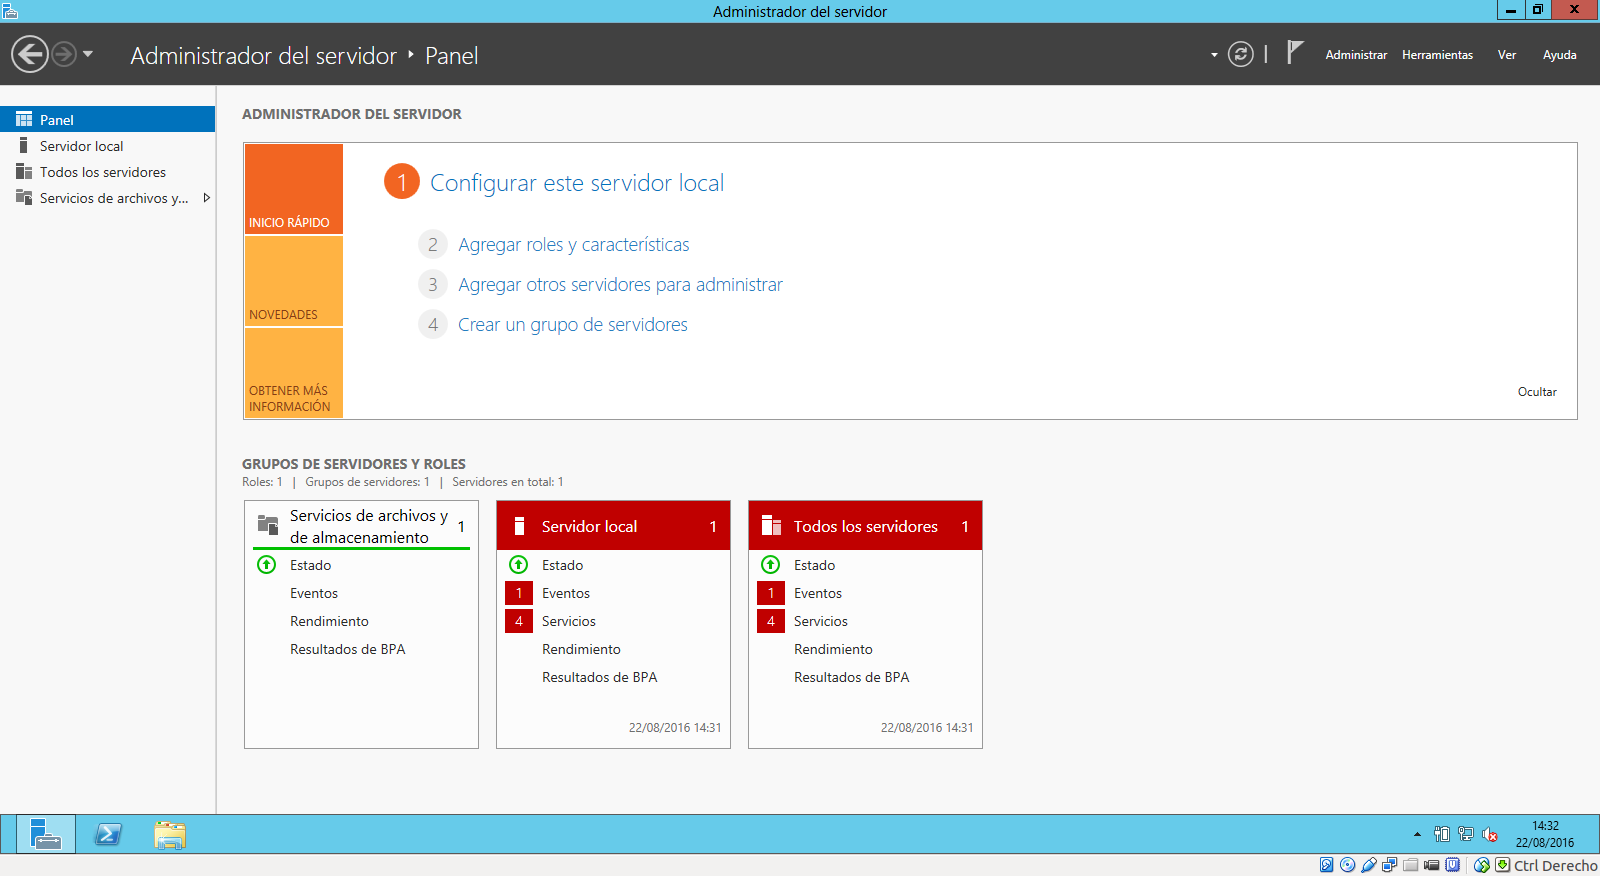
\includegraphics[width=0.7\linewidth]{WSAdministradorPanel}
		\caption[AdministradorPanel]{Panel de administrador de servicios de Windows.}
		\label{fig:WSAdministradorPanel}
	\end{figure}

	Clicamos en Agregar roles y características .\\
		
	\begin{figure}[H]
		\centering
		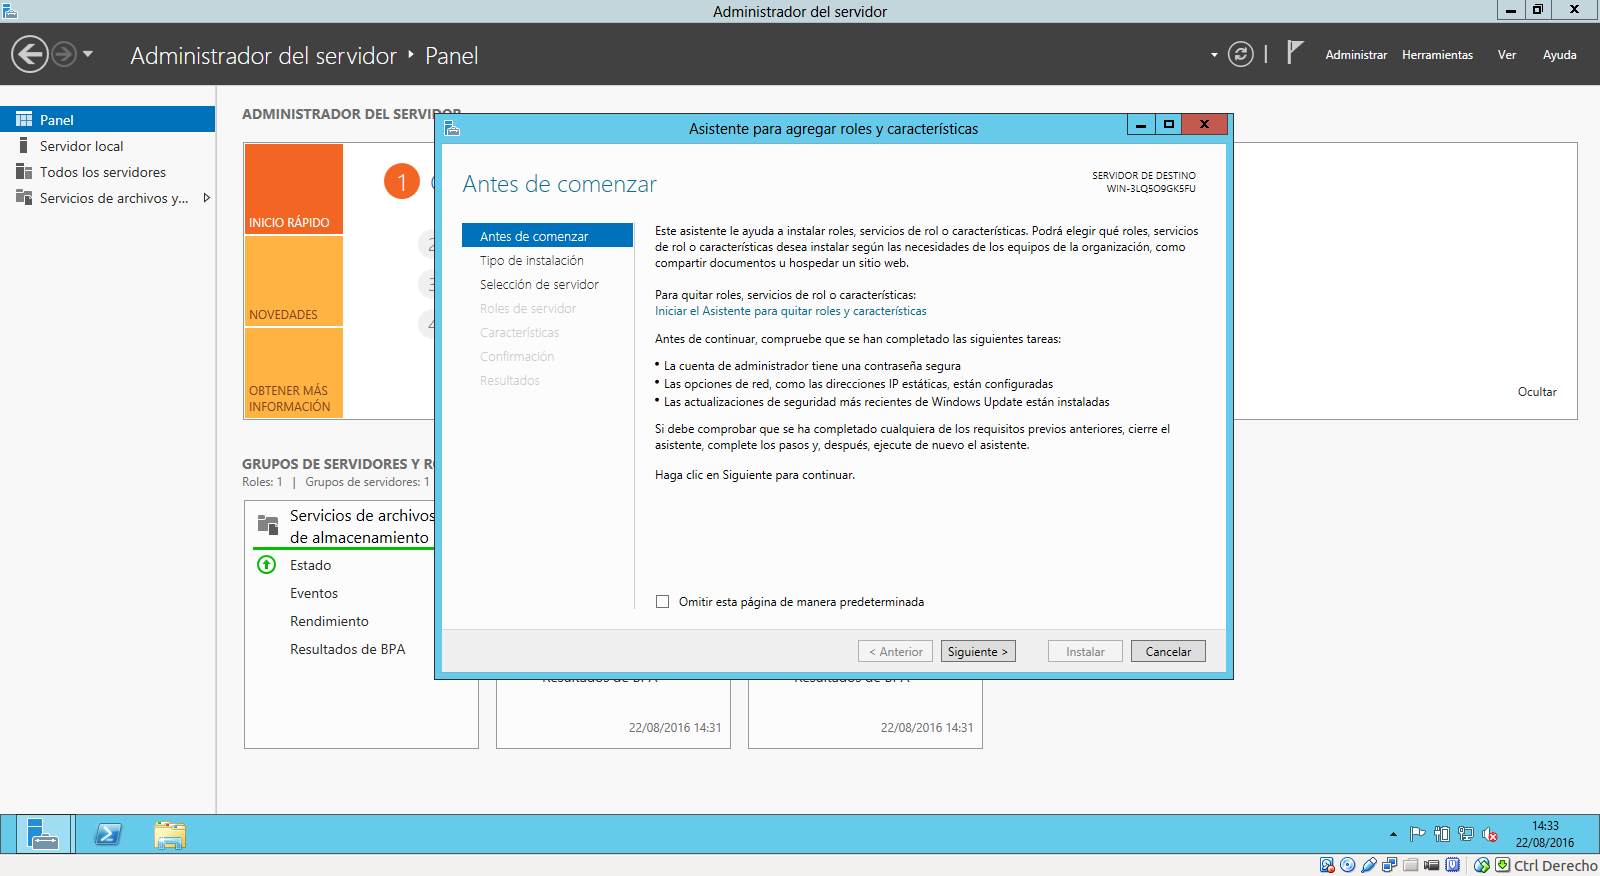
\includegraphics[width=0.7\linewidth]{AgregarRoles}
		\caption[Agregar roles]{Ventana inicial del asistente para agregar roles.}
		\label{fig:AgregarRoles}
	\end{figure}
	
	Entonces,tras pinchar Siguiente unas cuantas veces, seleccionamos el servicio IIS dicho anteriormente en el paso de Roles de servidor:\\
	
	\begin{figure}[H]
		\centering
		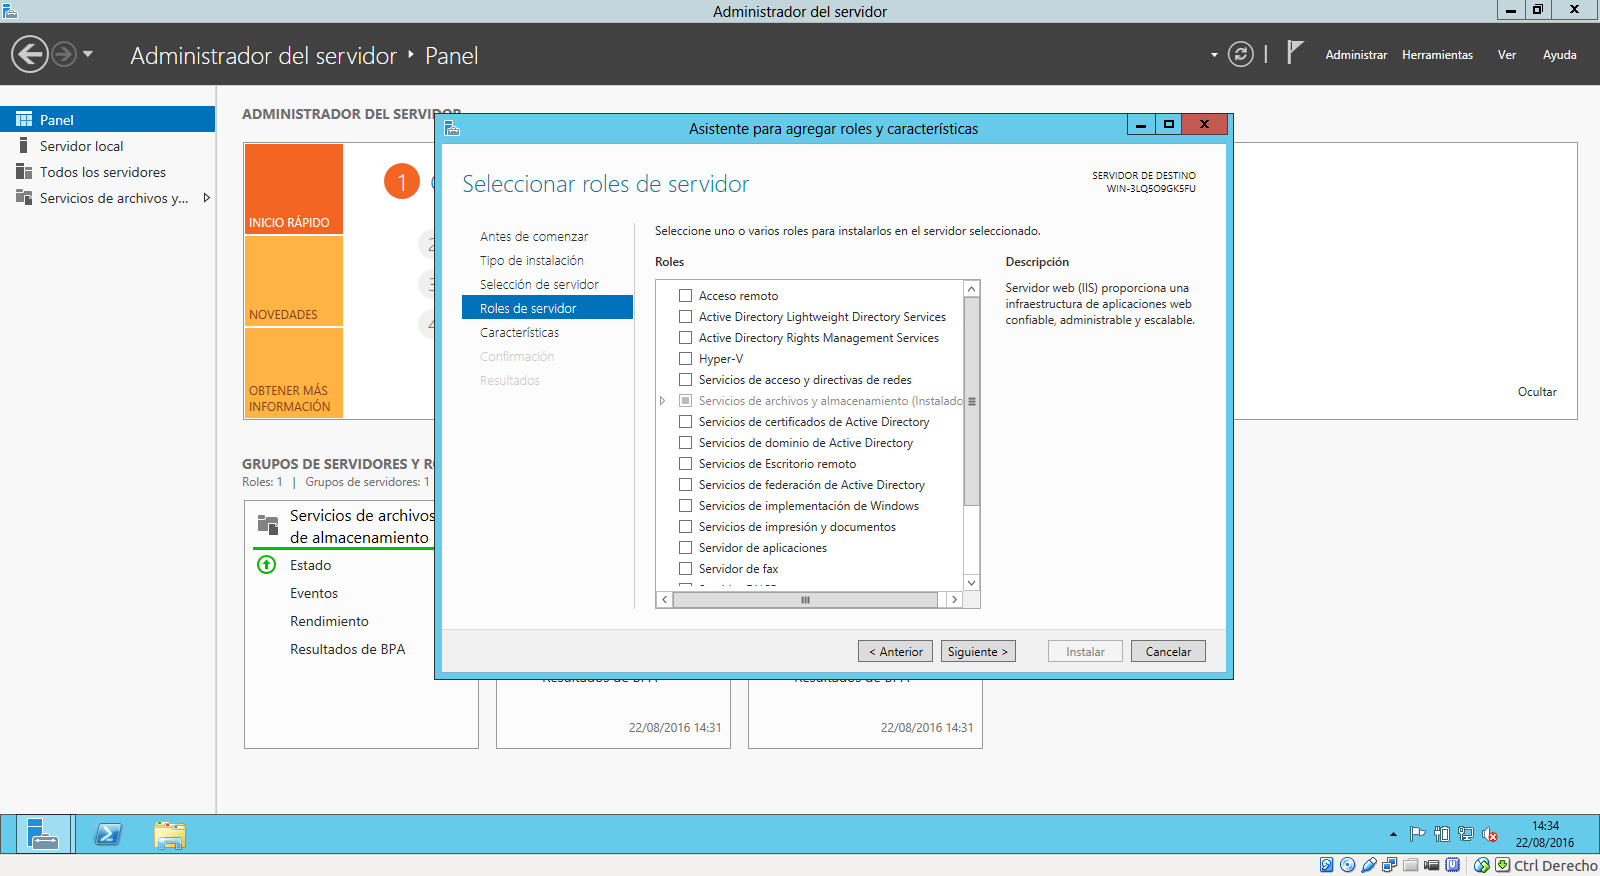
\includegraphics[width=0.7\linewidth]{SeleccionRoles}
		\caption[Selección de roles]{Lista de roles posibles en Windows. Buscamos el servicio IIS.}
		\label{fig:SeleccionRoles}
	\end{figure}
		
	Los servicios que debemos instalar tras esto, que son los servicios de “Estado y Diagnóstico”: “Herramientas de registro” y "Seguimiento". También instalaremos “Scripts y herramientas de administración de IIS” y el “Servicio de aministración”, que se encuentran en otra lista posterior:\\
		
	\begin{figure}[H]
		\centering
		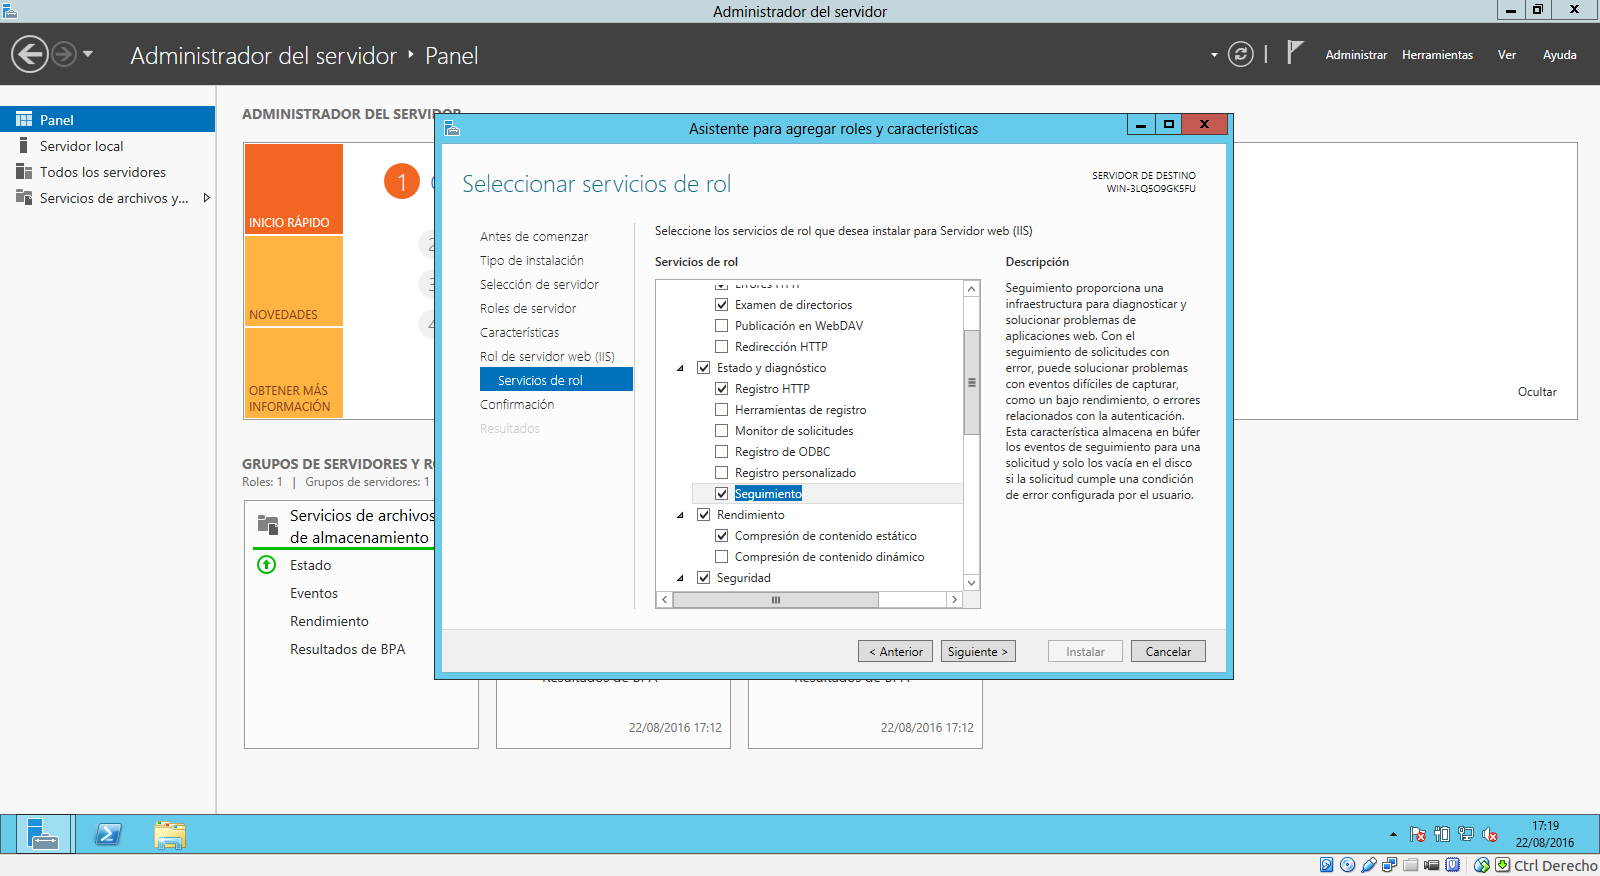
\includegraphics[width=0.7\linewidth]{ServiciosDeRol}
		\caption[Servicios de rol]{Servicios que ofrece el rol de IIS}
		\label{fig:ServiciosDeRol}
	\end{figure}
	
	Como último requisito para las prácticas, instalaremos FTP también:\\
		
	\begin{figure}[H]
		\centering
		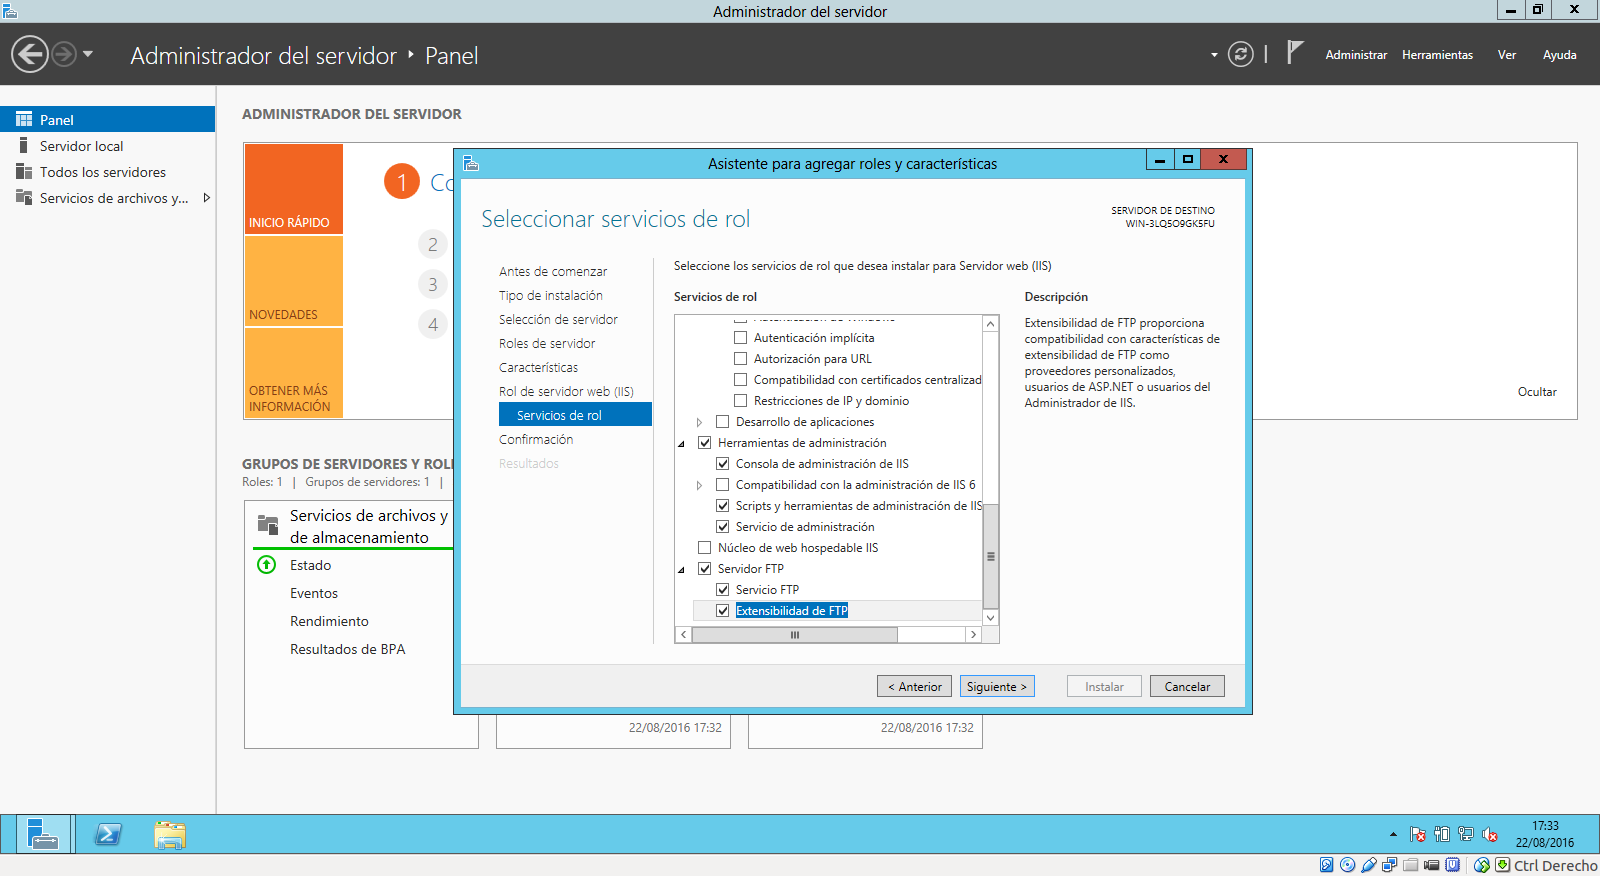
\includegraphics[width=0.7\linewidth]{FTPWS}
		\caption[Servicio FTP]{Servicio de rol FTP en Windows}
		\label{fig:FTPWS}
	\end{figure}
	
	Por último, se pide confirmación para la habilitación de servicios:\\
	
	\begin{figure}[H]
		\centering
		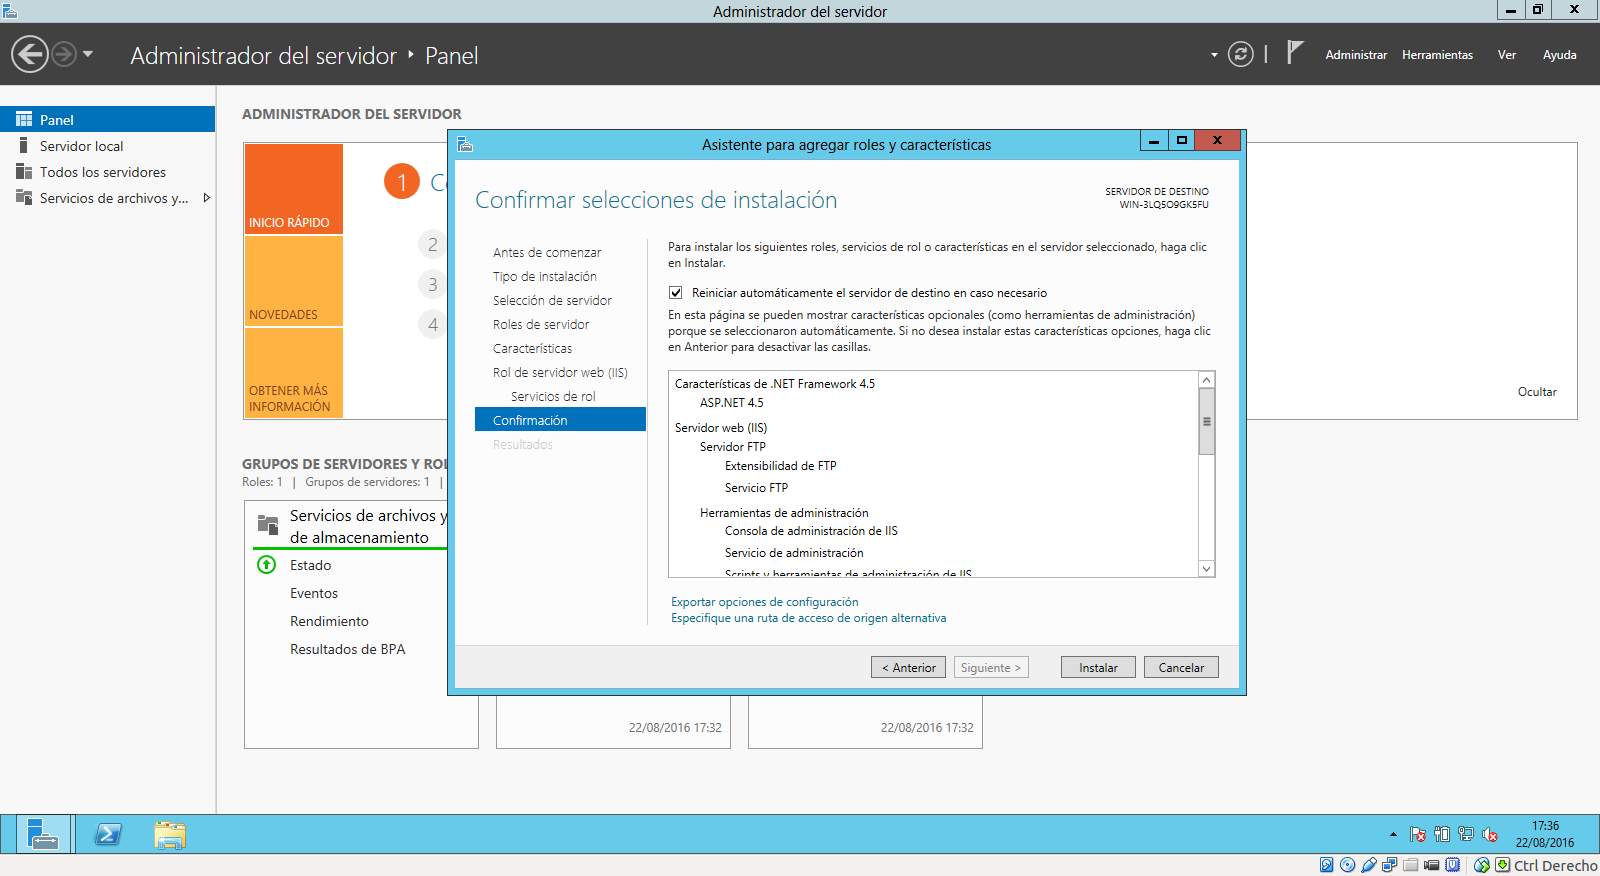
\includegraphics[width=0.7\linewidth]{ConfirmacionInstalacionWS}
		\caption[Confirmación Instalacion]{Confirmación para la instalación de los servicios.}
		\label{fig:ConfirmacionInstalacionWS}
	\end{figure}

	Ya tenemos el servidor apunto. Para comprobar que realmente funciona la página, accedemos desde otra máquina con entorno gráfico:\\
	
	\begin{figure}[H]
		\centering
		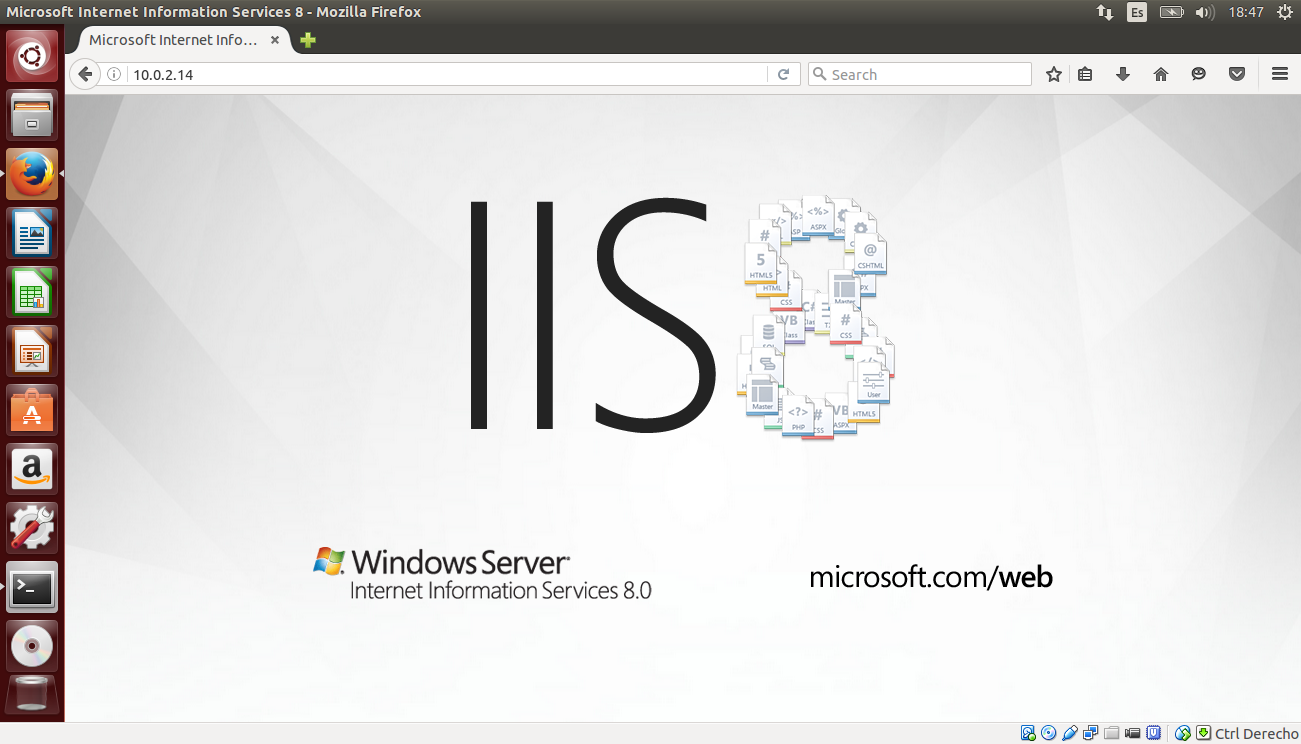
\includegraphics[width=0.7\linewidth]{WindowsWebPage}
		\caption[Pagina de web]{Pagina web con IIS como servidor web.}
		\label{fig:WindowsWebPage}
	\end{figure}
		
	Para habilitar ftp en Windows Server 2012 hay que seguir los siguientes pasos, sacados del servicio técnico de Microsoft\cite{tutorialFTP}:\\
	
	\begin{itemize}
		\item \textbf{Crear un usuario en el servidor Windows.}\\
		
		Para ello, en Panel de control->Cuentas de usuario->Administrar cuentas, clicamos en Agregar una cuenta de usuario. Rellenamos los campos de usuario, contraseña e indicio y ya tenemos creado nuestro usuario:\\
		
		\begin{figure}[H]
			\centering
			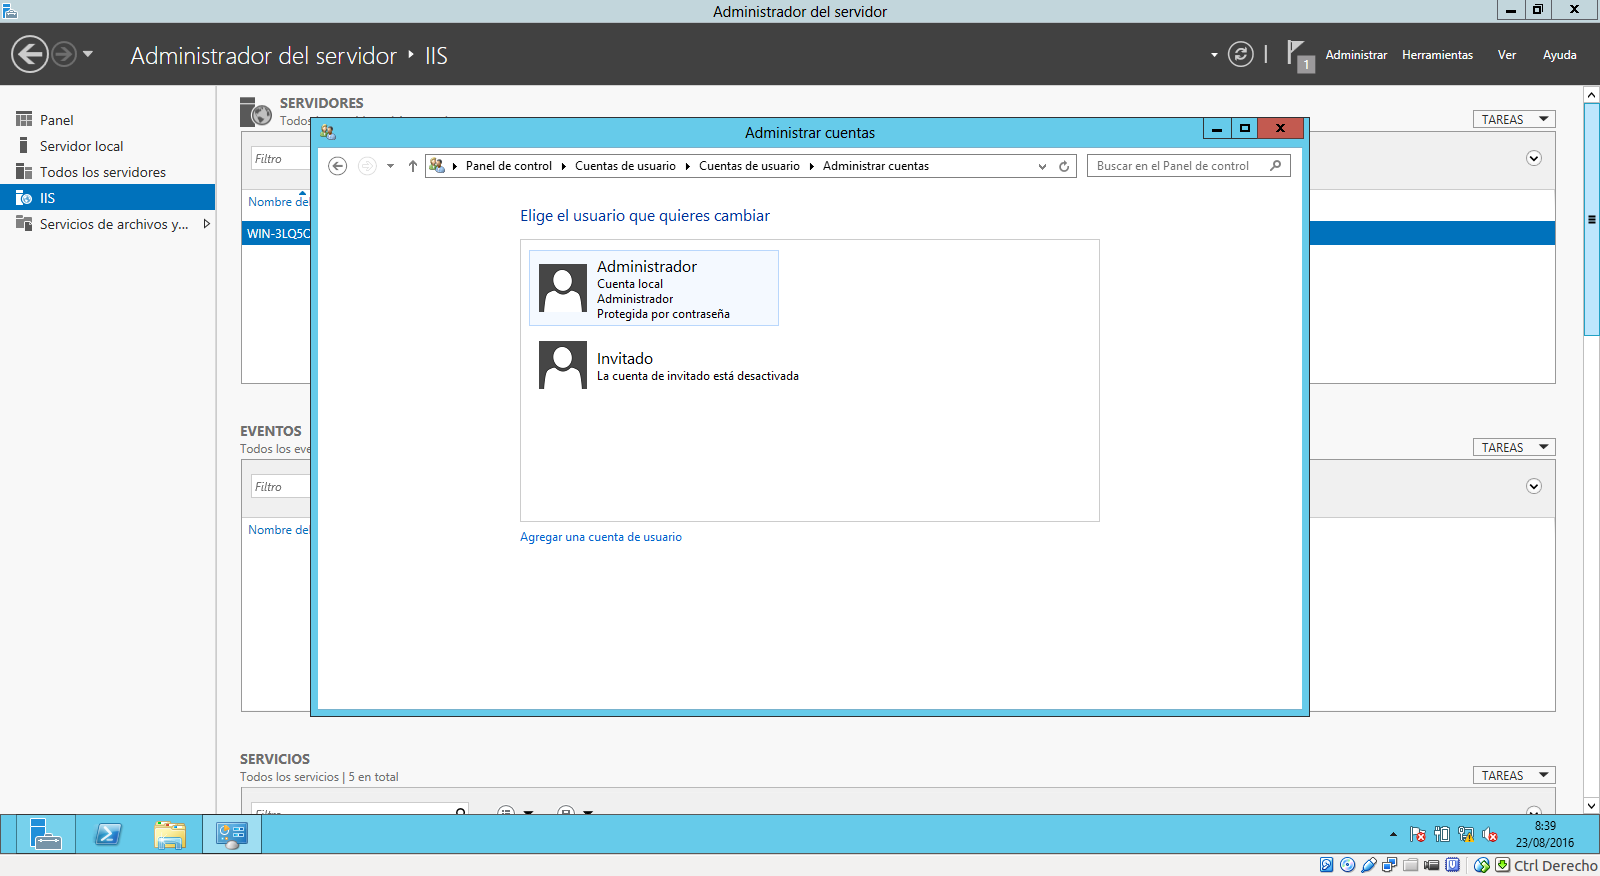
\includegraphics[width=0.7\linewidth]{AnadirCuentaUsuarioWS}
			\caption[Añadir cuenta]{Ventana en la que se encuentra el asistente para crear cuentas de usuario.}
			\label{fig:AñadirCuentaUsuarioWS}
		\end{figure}
		
		\item \textbf{Crear un sitio FTP al cual acceder.}\\
		
		Para ello, en el panel de administrador de roles, en la sección IIS, utilizamos la herramienta de administrador de IIS. Tras esto, expandimos el nodo conexiones y en el nodo sitios, aplicamos la acción Agregar sitio FTP. Un asistente de nos irá guiando en la creación del sitio FTP:\\
		
		\begin{figure}[H]
			\centering
			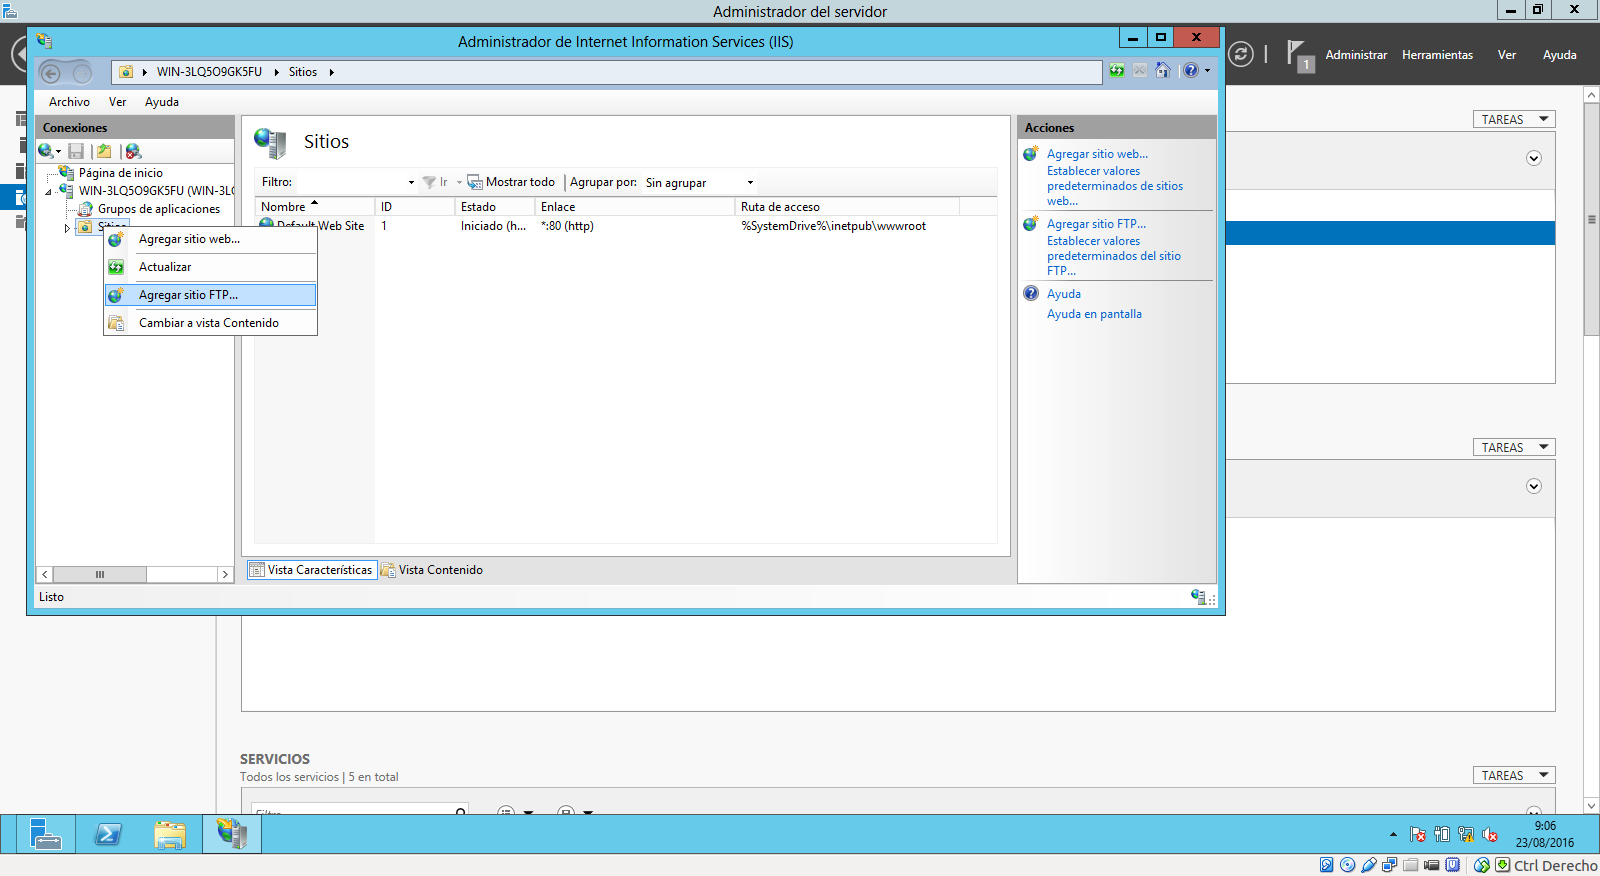
\includegraphics[width=0.7\linewidth]{AgregarSitioFTP}
			\caption[Agragar Sitio FTP]{Nodos a expandir para llamar al asistente de creación de sitio FTP.}
			\label{fig:AgregarSitioFTP}
		\end{figure}
			
		Tendremos que ponerle nombre a nuestro sitio y una ruta a la que acceder. En nuestro caso lo llamaremos ivan-ftp y lo localizaremos en la carpeta FTP en el disco C :\\
		
		\begin{figure}[H]
			\centering
			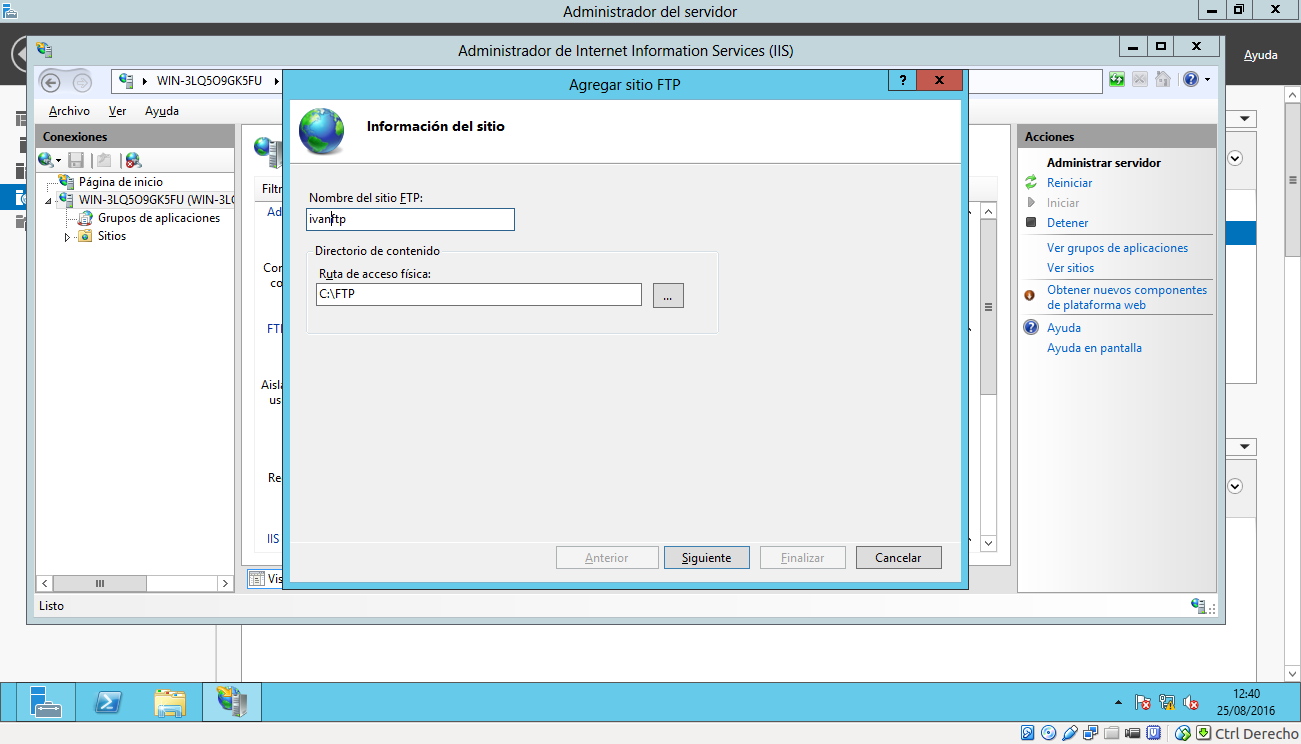
\includegraphics[width=0.7\linewidth]{WindowsServerDirectorioFtp}
			\caption[1\_SitioFTP]{Nombre y localización del sitio FTP.}
			\label{fig:NombreyLugarFTP}
		\end{figure}
		
		En la configuración de enlace y SSL, pinchamos en Sin SSl para no requerir el cifrado SSL. Los demás parámetros por defecto no será necesario modificarlos:\\
		
		\begin{figure}[H]
			\centering
			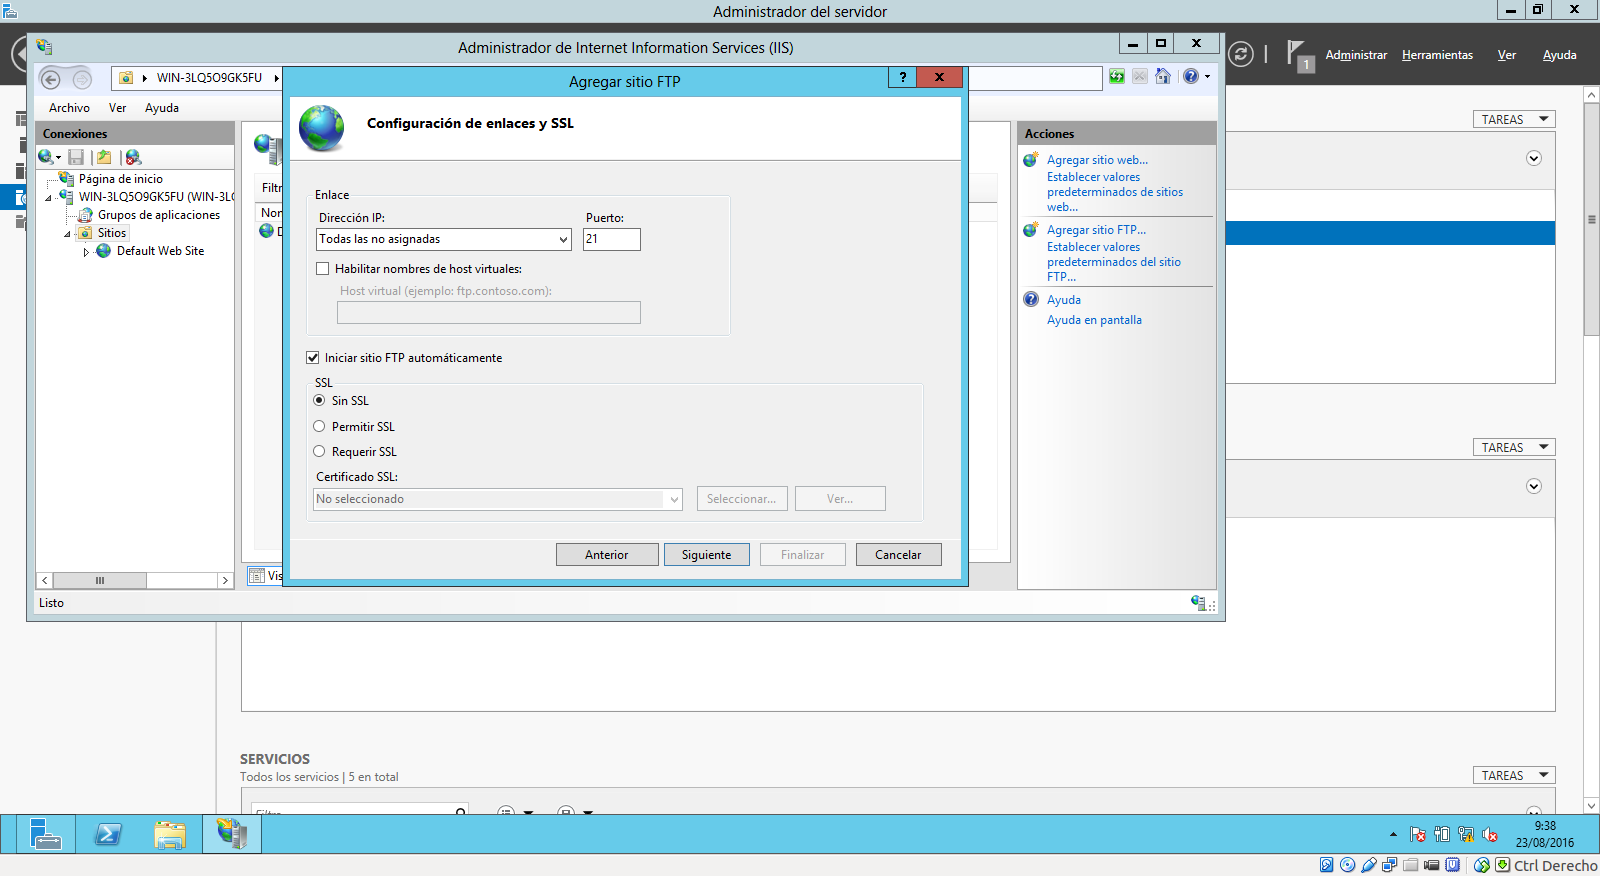
\includegraphics[width=0.7\linewidth]{ConfiguracionSSL}
			\caption[Configuración SSL]{Ventana de configuración de enlace y SSL.}
			\label{fig:ConfiguraciónSSL}
		\end{figure}
	 
	 Por último, incluimos al usuario ivan para que pueda leer y escribir los archivos del sitio FTP:\\
	 
	 \begin{figure}[H]
			\centering
			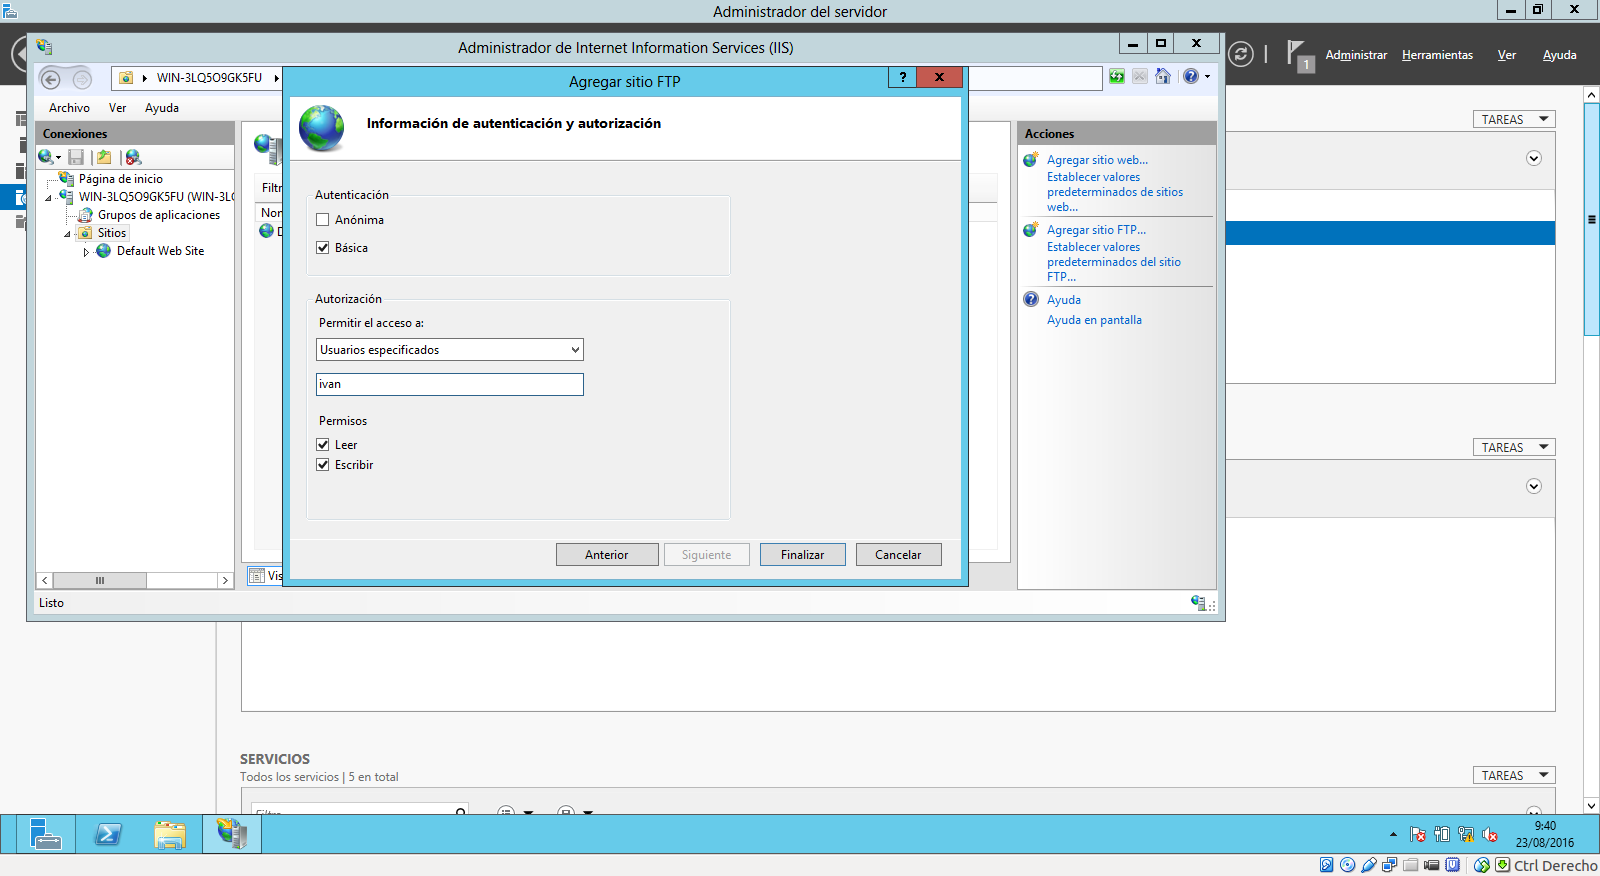
\includegraphics[width=0.7\linewidth]{PermisosFTP}
			\caption[Permisos FTP]{Añadir al usuario como lector y escritor del sitio FTP.}
			\label{fig:PermisosFTP}
		\end{figure}

		Así queda la configuración de sitios Web:\\
			
		\begin{figure}[H]
			\centering
			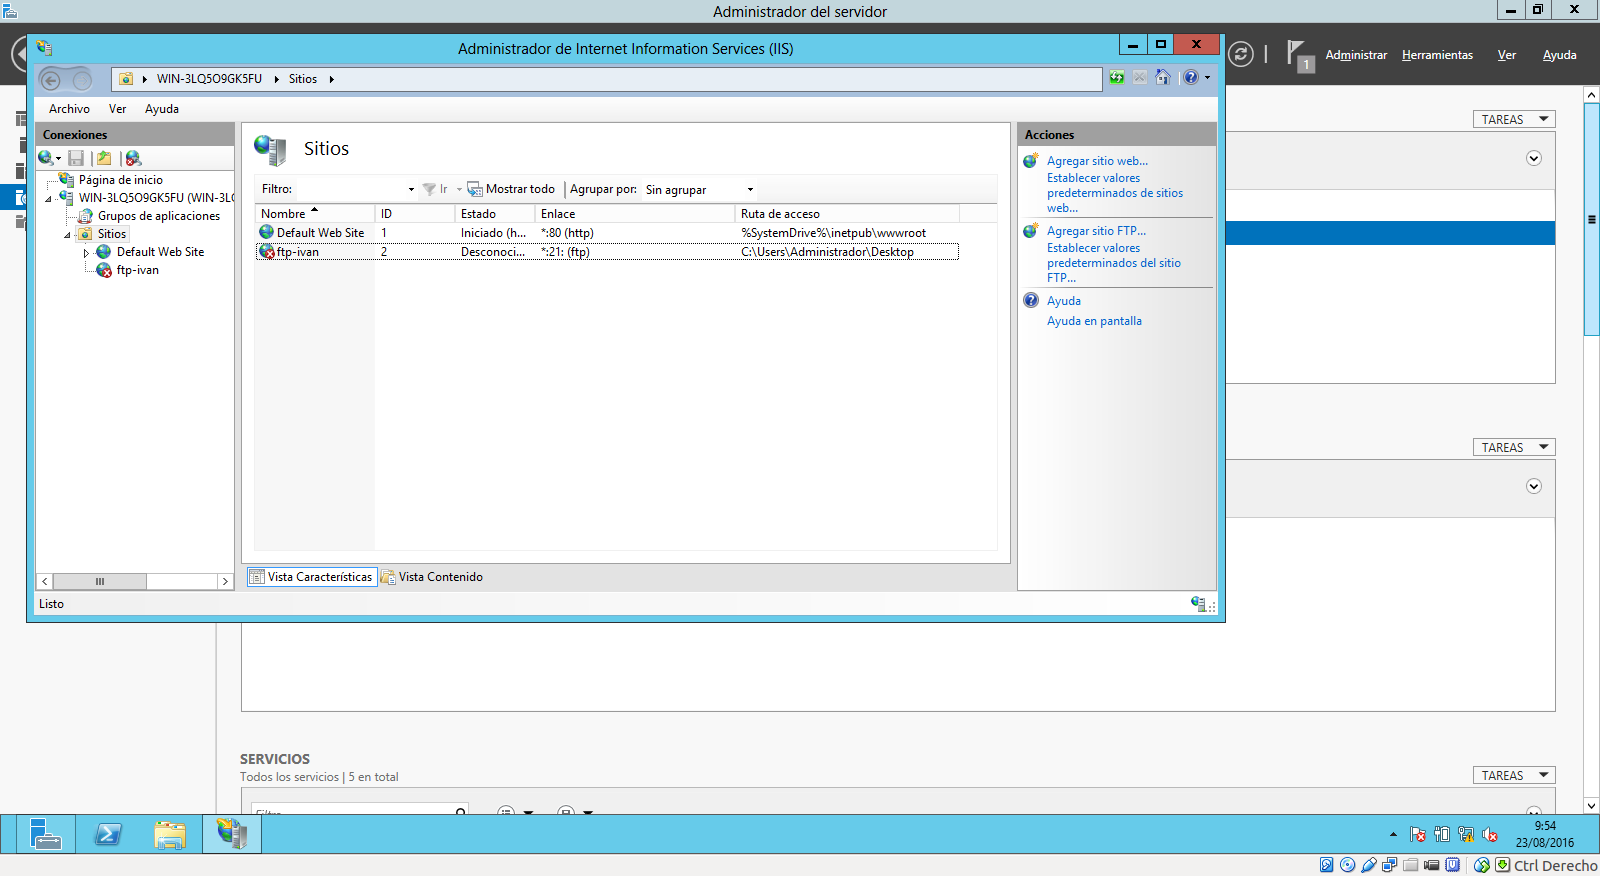
\includegraphics[width=0.7\linewidth]{ConfiguracionSitiosFinal}
			\caption[Configuracion sitios web final]{Configuración de sitios web tras la inclusión del sitio FTP.}
			\label{fig:ConfiguracionSitiosFinal}
		\end{figure}
		
		\item \textbf{Modificar el firewall de Windows para que la conexión ftp pueda llevarse a cabo.}\\
		
		La herramienta firewall se encuentra en Herramientas Administrativas. Solo hay que añadir una regla de entrada que acepte las peticiones al puerto 21, el puerto por defecto de FTP. Para ello, abrimos el FireWall de Windows y creamos una regla de entrada en la que se acepte la conexión. La conexión se llevará a cabo a través del puerto 21. El asistente tiene las siguientes ventanas, explicadas en su descripción:\\
			
		\begin{figure}[H]
			\centering
			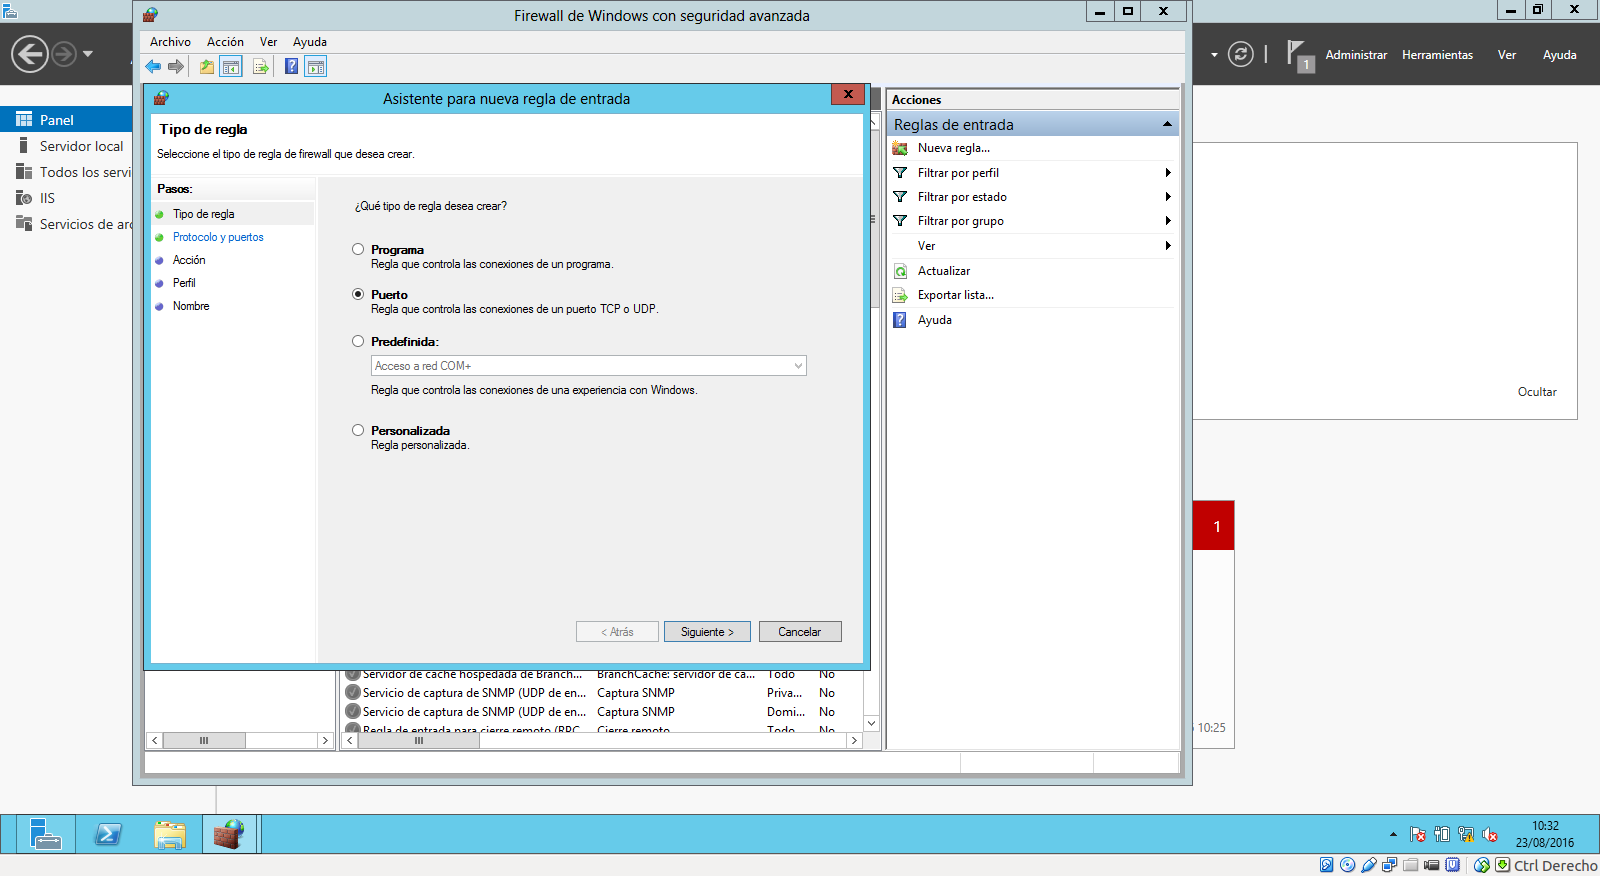
\includegraphics[width=0.7\linewidth]{TipoReglaPuerto}
			\caption[Tipo de regla]{Tipo de regla que vamos a crear. Se elije la configuración puerto, ya que para que se escuche las peticiones ftp, vasta que se abra el puerto 21.}
			\label{fig:TipoReglaPuerto}
		\end{figure}
		
		\begin{figure}[H]
			\centering
			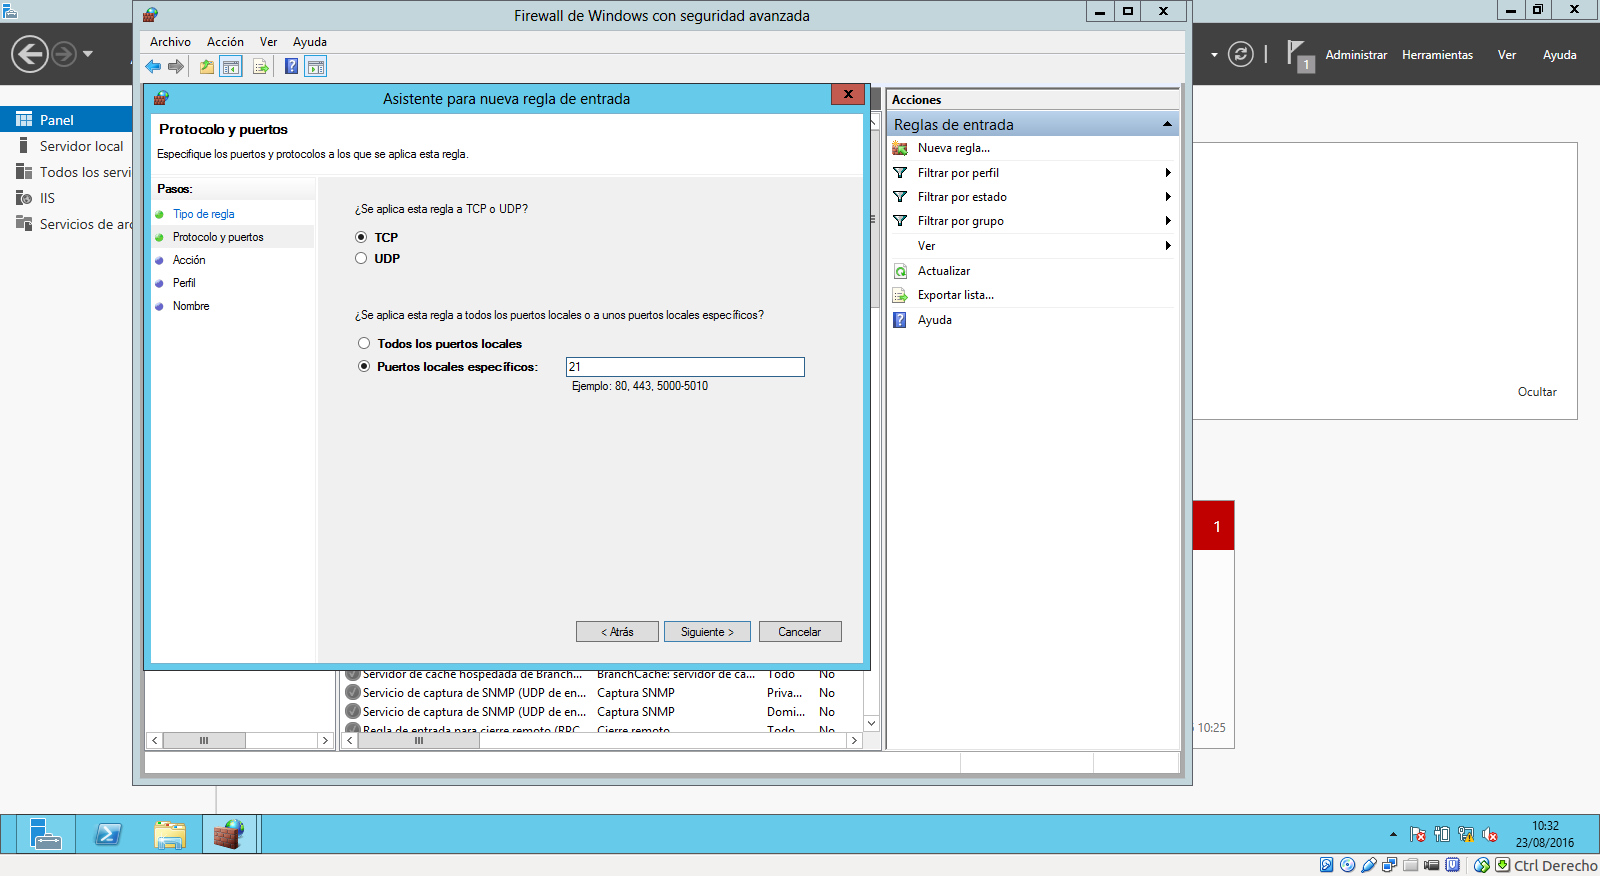
\includegraphics[width=0.7\linewidth]{Puerto21}
			\caption[Puerto seleccionado]{Selección del protocolo a seguir y el puerto que se va a abrir. Escogemos TCP y el puerto 21.}
			\label{fig:Puerto21}
		\end{figure}
			
		\begin{figure}[H]
			\centering
			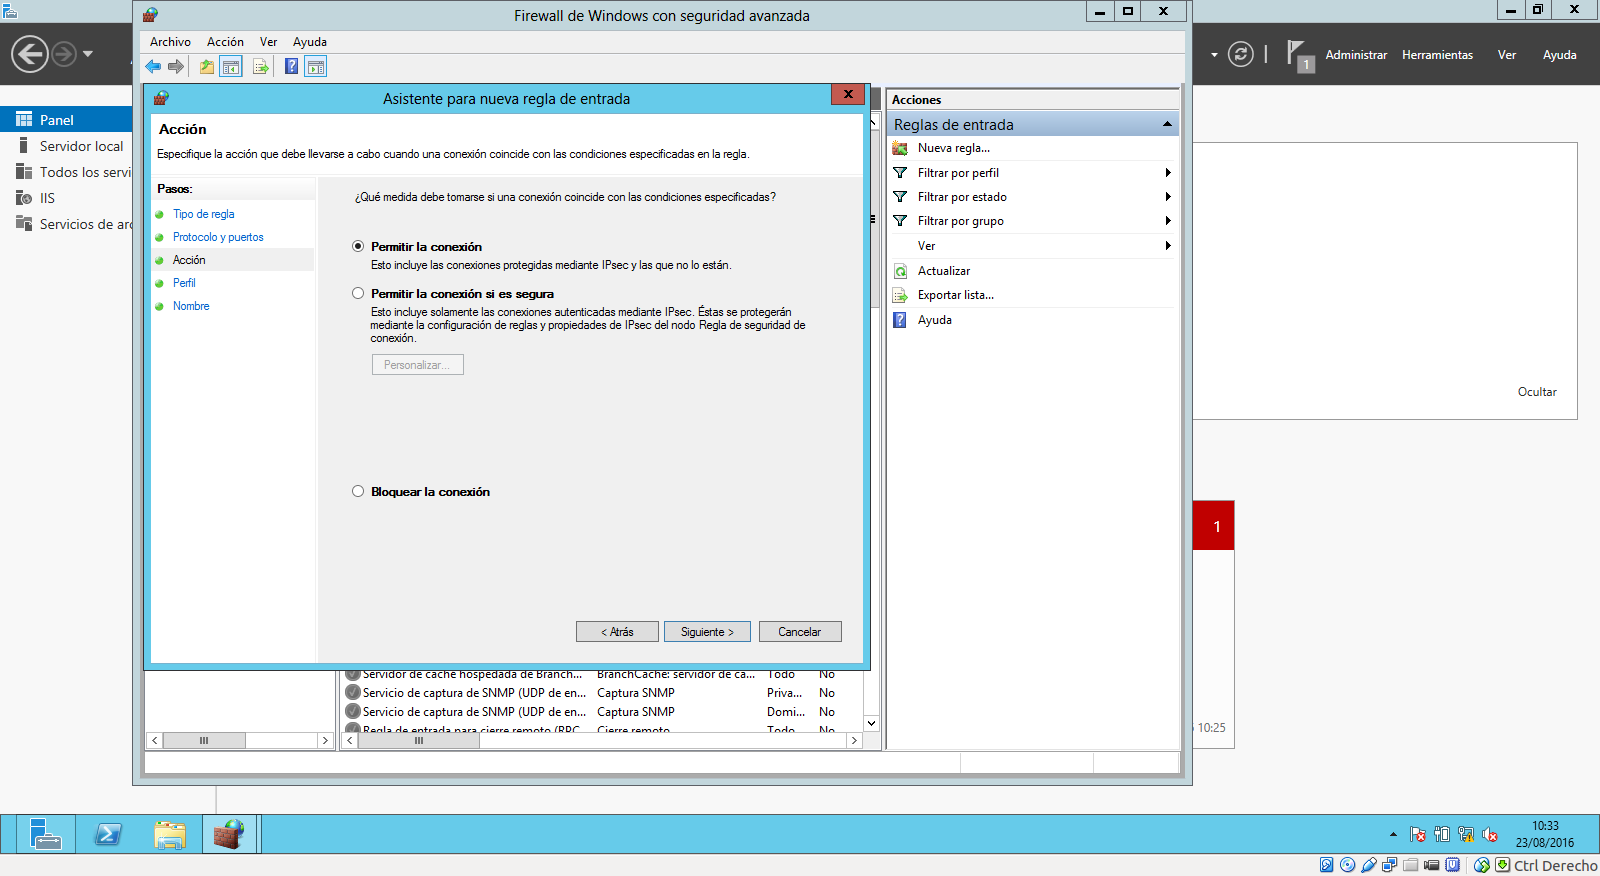
\includegraphics[width=0.7\linewidth]{PermitirConexionFTP}
			\caption[Permitir conexión]{Acción a realizar. Marcamos la opción de permitir la conexión ftp.}
			\label{fig:PermitirConexionFTP}
		\end{figure}
		
		Tras estas ventanas, tenemos que ponerle nombre y añadir una descripción a la regla. No creo necesario incluir captura de pantalla de esta parte. Ya tenemos la regla de entrada configurada. Solo queda comprobar que funciona. Realizaremos ahora la conexión ftp desde otra máquina:\\
		
		
		
			
	\end{itemize}

\end{itemize}	
	
\section{Manteniendo los servicios actualizados}
\begin{itemize}
	\item \textbf{Ejemplo de uso de el comando patch.} Muestre un ejemplo de uso del comando patch, por ejemplo en el link dado en la referencia \cite{patch}.\\

	Existe un comando, diff\cite{diff}, el cual extrae la diferencia entre dos archivos y lo codifica en un archivo .diff. El comando patch\cite{patch} sirve para aplicar esos cambios a uno de los archivos para cambiarlo al otro. Esto es muy útil, ya que si se ha distribuido una versión de un código compilado con un error no detectado, no vamos a volver a distribuir de nuevo el ejecutable entero, si no que obtendremos con diff la diferencia entre el código original con errores y el nuevo código y pediremos que se aplique este parche al código compilado.
	
	En el link se explica como instalar VMWare. En el mismo se contemplan varios errores, entre ellos uno en el que se le puede aplicar un parche descargable. Esto se soluciona al aplicar el comando patch. Mostramos aquí el script que ofrecen para solucionarlo:\\
	
	// Descarga del parche en un directorio temporal:\\
	\$ curl http://pastie.org/pastes/8672356/download -o /tmp/vmware-netfilter.patch\\
	
	// Cambio del directorio y descompresión del archivo a modificar.\\
	\$ cd /usr/lib/vmware/modules/source\\
	\# tar -xvf vmnet.tar\\
	
	// Aplicación del parche.\\
	\# patch -p0 -i /tmp/vmware-netfilter.patch\\
	
	// Compresión del archivo modificado\\
	\# tar -cf vmnet.tar vmnet-only\\
	
	// Instalar lo que quedaba de VMWare.\\
	\# rm -r vmnet-only\\
	\# vmware-modconfig --console --install-all\\

\end{itemize}

\section{Administración web.}

\begin{itemize}
	\item \textbf{Realice la instalación de webadmin y pruebe a modificar algún parámetro de algún servicio. Muestre las capturas de pantalla pertinentes así como el proceso de instalación.}\\
	
	Para instalar webadmin vamos a seguir los pasos detallados en la página de webadmin para la instalación de paquetes\cite{webadminInstalation}:\\
	
	Primero debemos modificar el archivo $/etc/apt/sources.list$ y añadir la siguiente linea:\\
	
	deb http://download.webmin.com/download/repository sarge contrib\\
	
	\begin{figure}[H]
		\centering
		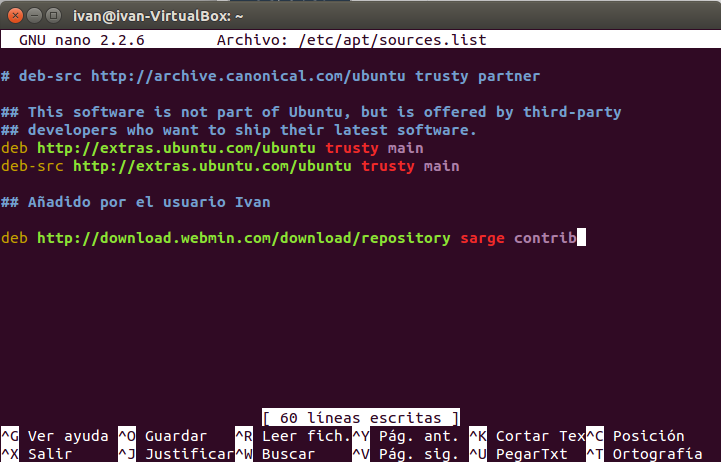
\includegraphics[width=0.7\linewidth]{AnadirRepo}
		\caption[AñadirRepo]{Repositorio añadido a apt.}
		\label{fig:AñadirRepo}
	\end{figure}
	
	Tras lo cual debemos instalar la clave para poder descargar el paquete:\\
	
	cd /root\\
	wget http://www.webmin.com/jcameron-key.asc\\
	apt-key add jcameron-key.asc\\
	
	\begin{figure}[H]
		\centering
		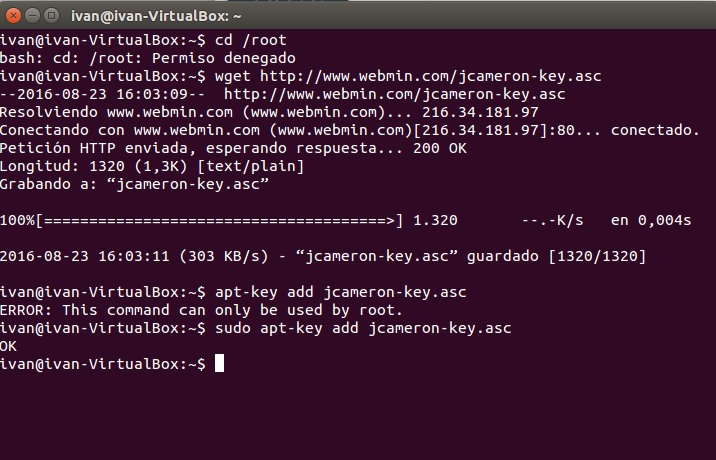
\includegraphics[width=0.7\linewidth]{AnadirClave}
		\caption[Añadir clave]{Añadir la clave necesaria para instalar webadmin}
		\label{fig:AnadirClave}
	\end{figure}

	
	Una vez hecho esto, se puede instalar webmin desde repositorio, para lo cual antes tenemos que actualizar la lista de paquetes(apt update) e instalar el paquete de webadmin:\\
	
	\begin{figure}[H]
		\centering
		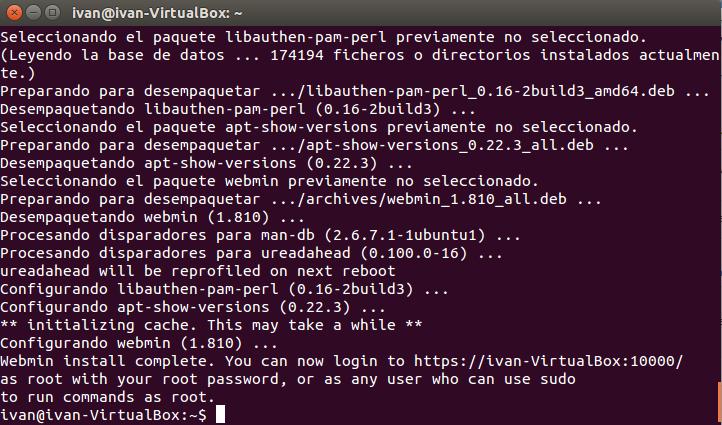
\includegraphics[width=0.7\linewidth]{WebminInstalled}
		\caption[Webmin Instalado]{Instalación de webmin llevada a cabo a través de repositorio.}
		\label{fig:WebminInstalled}
	\end{figure}
	
	Aquí vemos Webadmin accesible en el puerto 10000 del servidor:\\
	
	\begin{figure}[H]
		\centering
		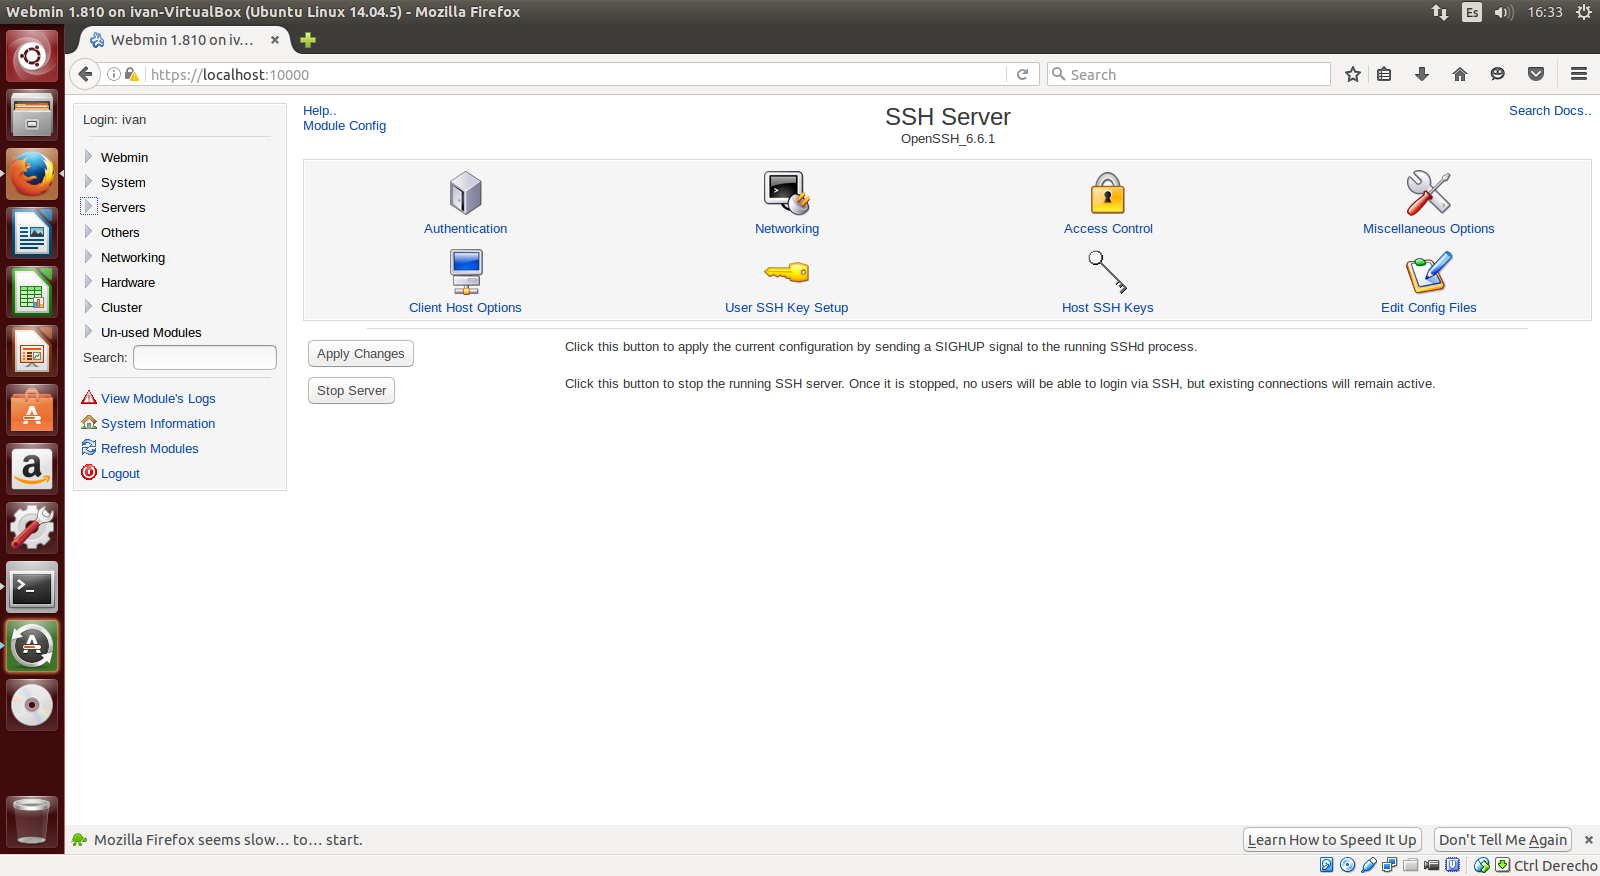
\includegraphics[width=0.7\linewidth]{WebminAccesible}
		\caption[Webmin accesible]{Webmin accesible en el navegador. Por defecto, escucha el puerto 10000.}
		\label{fig:WebminAccesible}
	\end{figure}

	Se nos pide que modifiquemos algún parámetro de algún servicio y mostremos que funciona. Nosotros modificaremos el puerto de escucha del servidor de apache. Para ello, extendemos el nodo Servers y seleccionamos la configuración global de Apache:\\
	
	\begin{figure}[H]
		\centering
		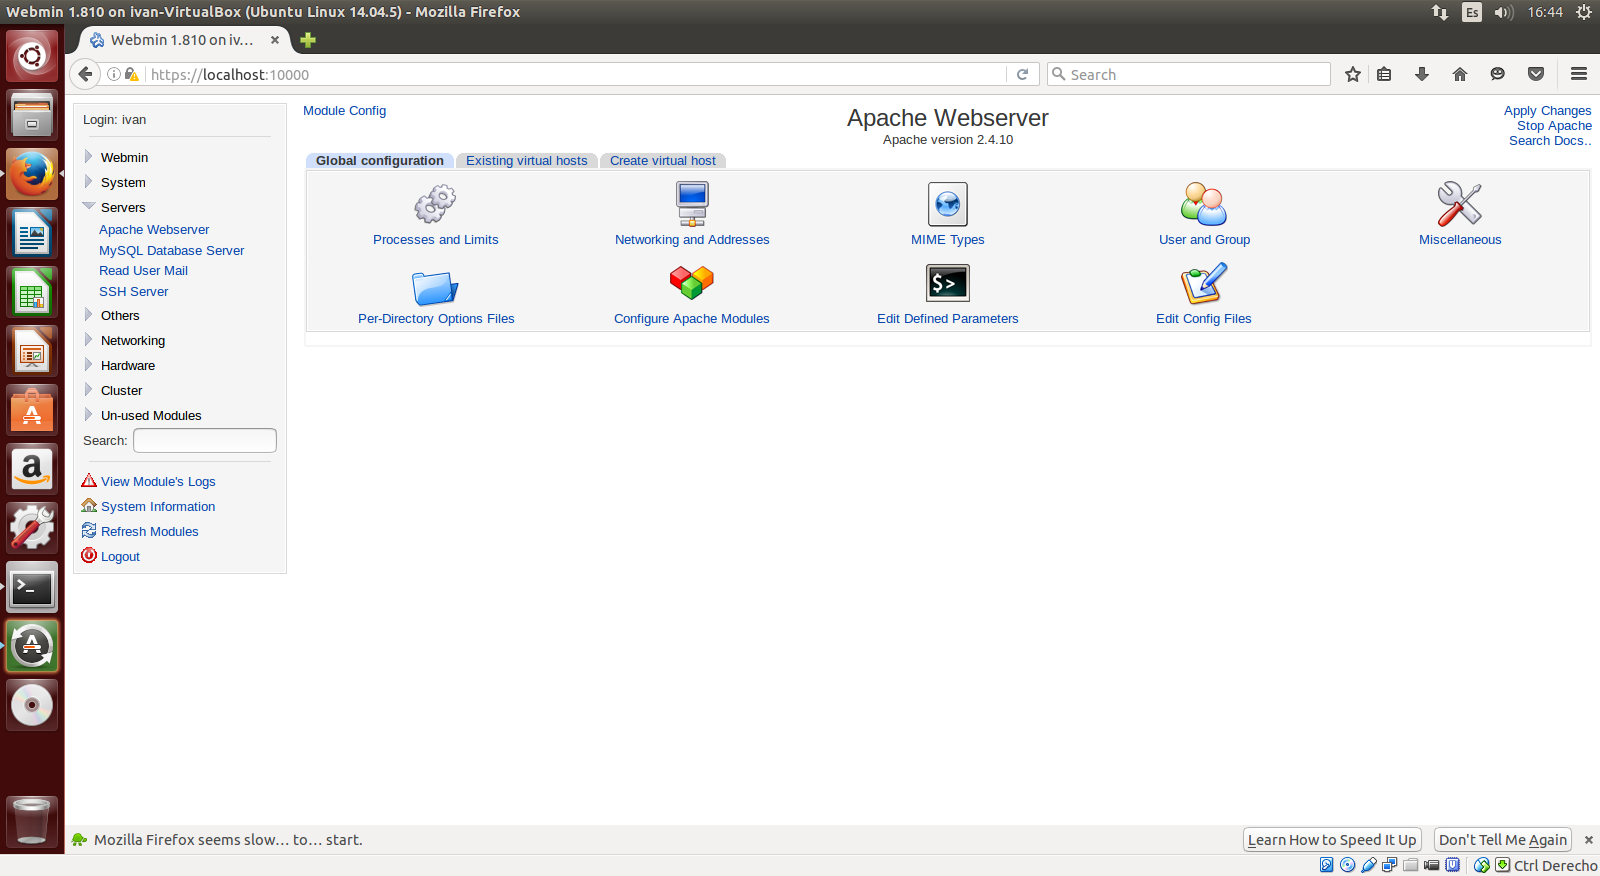
\includegraphics[width=0.7\linewidth]{WebminApacheGlobalConf}
		\caption[Configuracion global apache]{Configuración global de Apache ofrecida por Webmin.}
		\label{fig:WebminApacheGlobalConf}
	\end{figure}
	
	donde seleccionaremos redes y direcciones(Network and Addresess). Entonces, en la casilla del puerto de escucha, cambiamos a 8080:\\
	
	\begin{figure}[H]
	\centering
	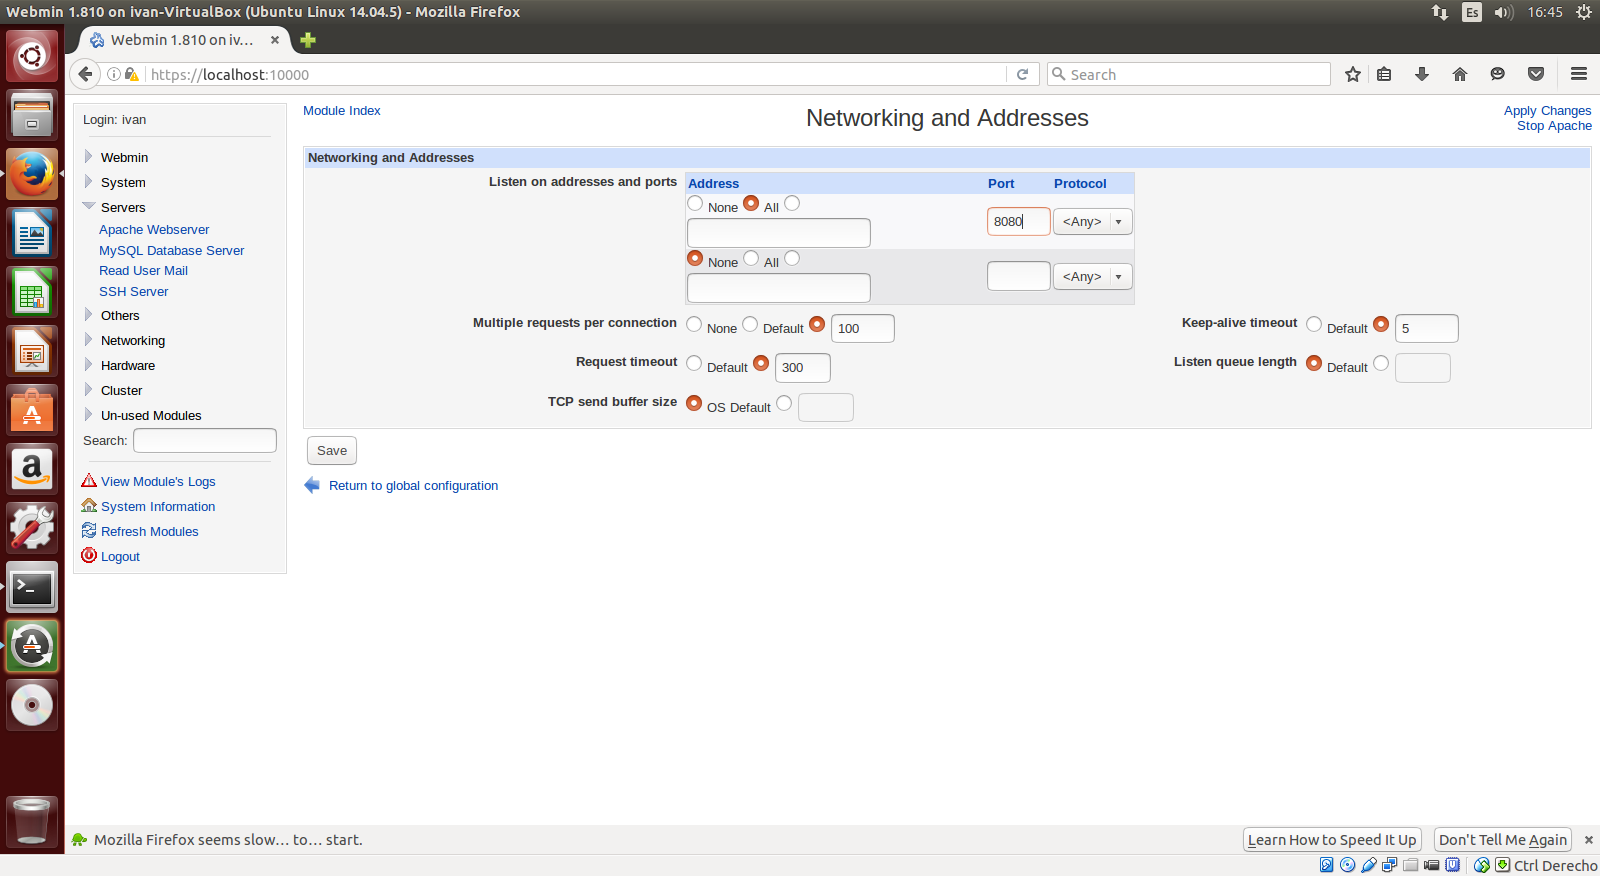
\includegraphics[width=0.7\linewidth]{WebminPuertoCambiado}
	\caption[Modificacion Puerto]{Puerto del servicio Apache modificado por Webmin al 8080.}
	\label{fig:WebminPuerto8080}
	\end{figure}
	
	Al guardar y aplicar los cambios, vemos que podemos acceder a la página web de Apache en el puerto 8080:\\
	
	\begin{figure}[H]
		\centering
		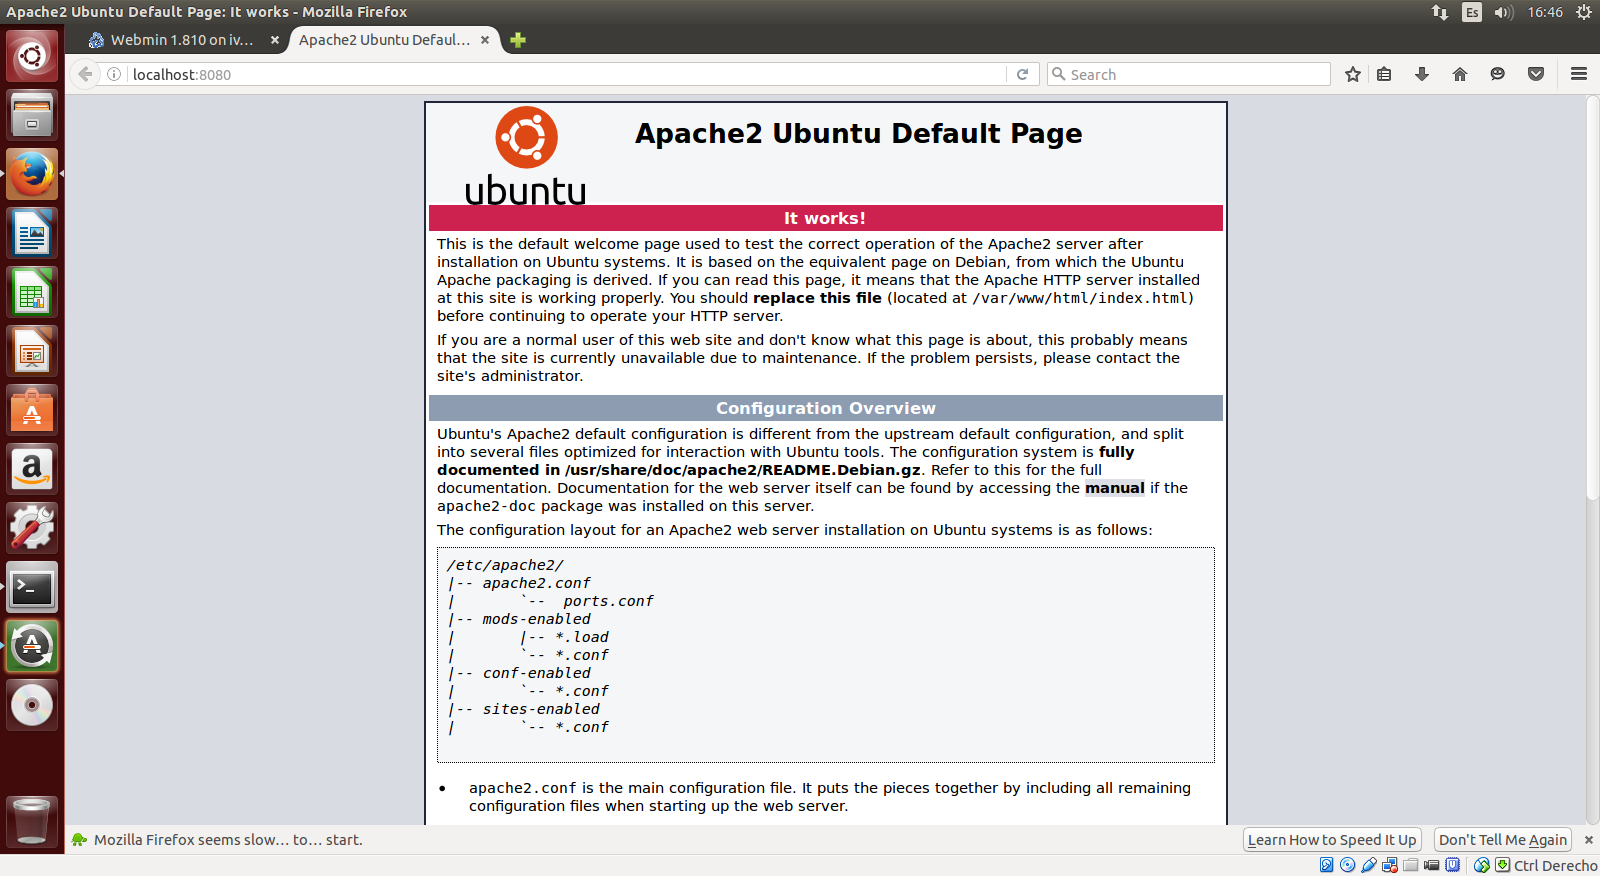
\includegraphics[width=0.7\linewidth]{WebminPuerto8080}
		\caption[Puerto cambiado 2]{Página de apache ofrecida en el puerto 8080.}
		\label{fig:WebminPuertoCambiado}
	\end{figure}

	\item \textbf{Instale phpMyAdmin, indique cómo lo ha realizado y muestre algunas capturas de pantalla. Configure PHP para poder importar BDs mayores de 8MiB (límite por defecto). Indique cómo ha realizado el proceso y muestre capturas de pantalla.}\\
	
	Según la página oficial de phpMyAdmin\cite{phpMyAdmin}, podemos añadir el repositorio escribiendo el siguiente comando:\\
	
	$sudo$ $add$-$apt$-$repository$ $ppa$:$nijel$/$phpmyadmin$\\
	
	así que tras actualizar el sistema(apt-get update), debemos de tener el paquete phpmyadmin en la lista de paquetes que podemos descargar. Ejecutamos el siguiente comando:\\
	
	$sudo$ $apt$ $install$ $phpmyadmin$
	
	el cual nos dejará configurar algunas opciones de phpmyadmin mientras se instala:\\
	
	\begin{figure}[H]
		\centering
		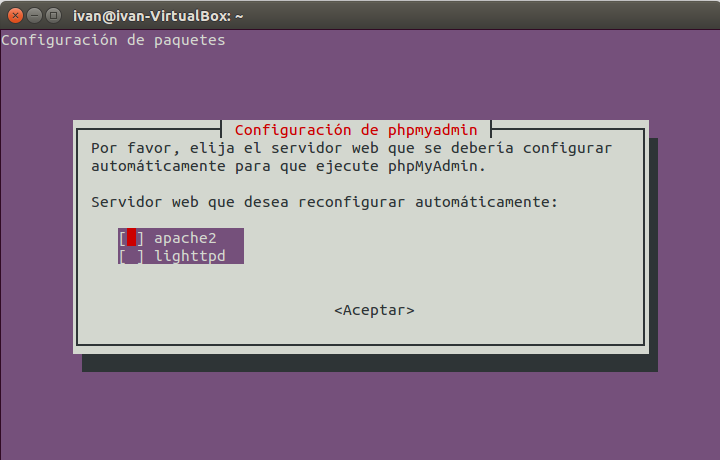
\includegraphics[width=0.7\linewidth]{phpMyAdminApache2}
		\caption[Phpmyadmin]{Servidor web que configurar por defecto. Nosotros elegiremos apache2.}
		\label{fig:phpMyAdminApache2}
	\end{figure}
	
	\begin{figure}[H]
		\centering
		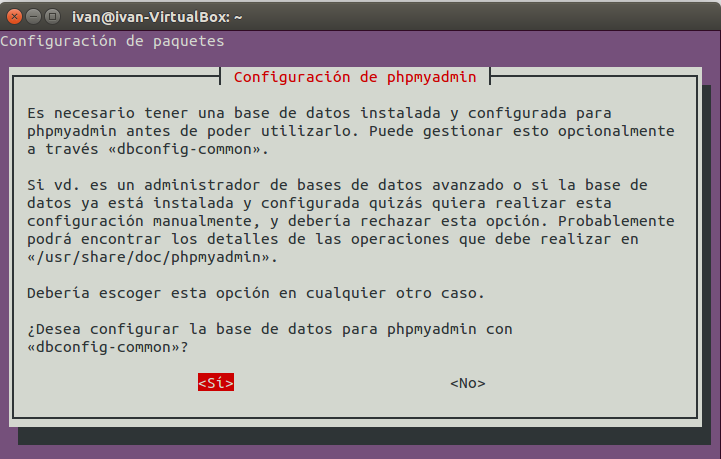
\includegraphics[width=0.7\linewidth]{phpmyadminConfPorDefecto}
		\caption[Configuración por defecto.]{Configuración por defecto para la base de datos. Por defecto, y como no somos expertos en la materia, tendremos esta configuración.}
		\label{fig:phpmyadminConfPorDefecto}
	\end{figure}
	
	\begin{figure}[H]
		\centering
		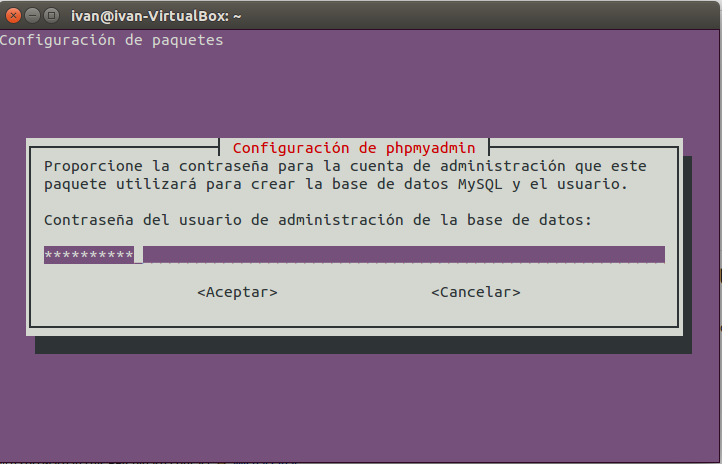
\includegraphics[width=0.7\linewidth]{PhpMyadminContrasenaBaseDatos}
		\caption[Contraseña base de datos]{Configurar la contraseña para la base de datos.}
		\label{fig:PhpMyadminContraseñaBaseDatos}
	\end{figure}
	
	\begin{figure}[H]
		\centering
		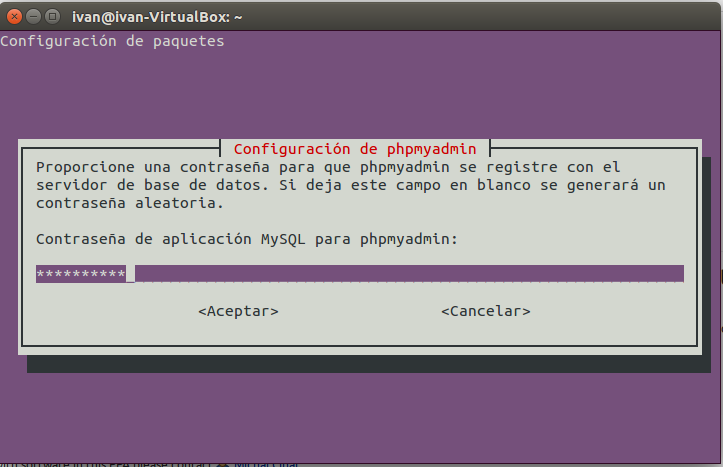
\includegraphics[width=0.7\linewidth]{PhpmyadminContrasena2}
		\caption[Contraseña 2 phpmyadmin]{Contraseña que pide phpmyadmin para la base de datos.}
		\label{fig:PhpmyadminContraseña2}
	\end{figure}
	
	Ya tenemos instalada la herramienta PhpMyAdmin. Para acceder a ella en un navegador accedemos a la dirección $localhost/phpmyadmin$ :\\
	
    \begin{figure}[H]
		\centering
		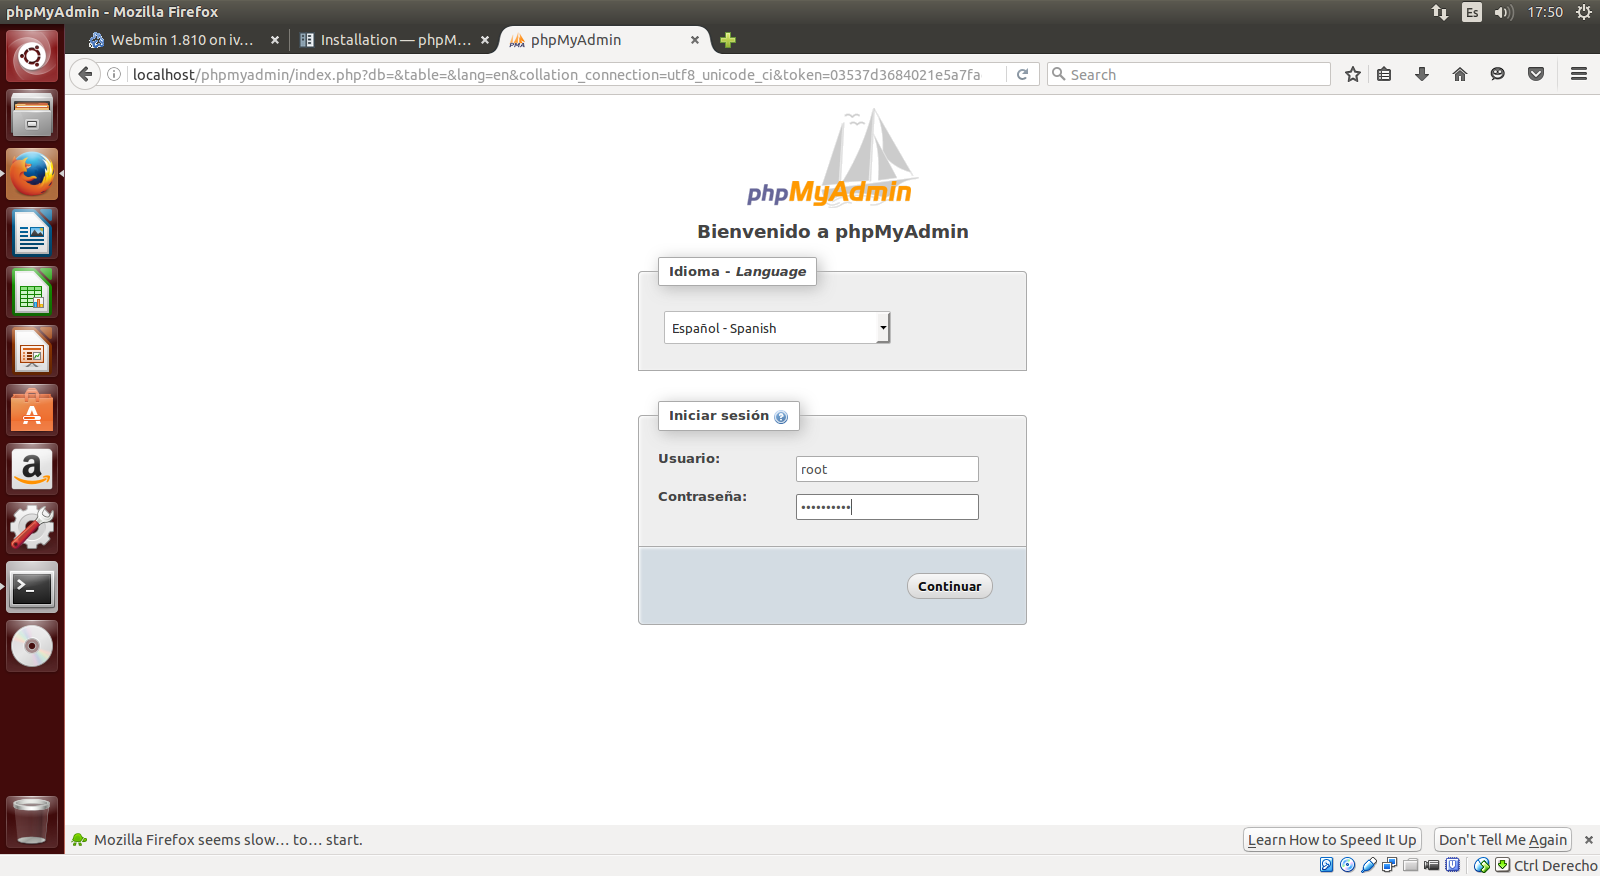
\includegraphics[width=0.7\linewidth]{PHPMyadminpantallaInicio}
		\caption[Phpmyadmin pantalla inicio]{Pantalla de inicio de PhpMyAdmin}
		\label{fig:PHPMyadminpantallaInicio}
	\end{figure}
	
	La siguiente es la página de inicio que se abre tras autenticarse como usuario root de phpmyadmin:\\
	
	\begin{figure}[H]
		\centering
		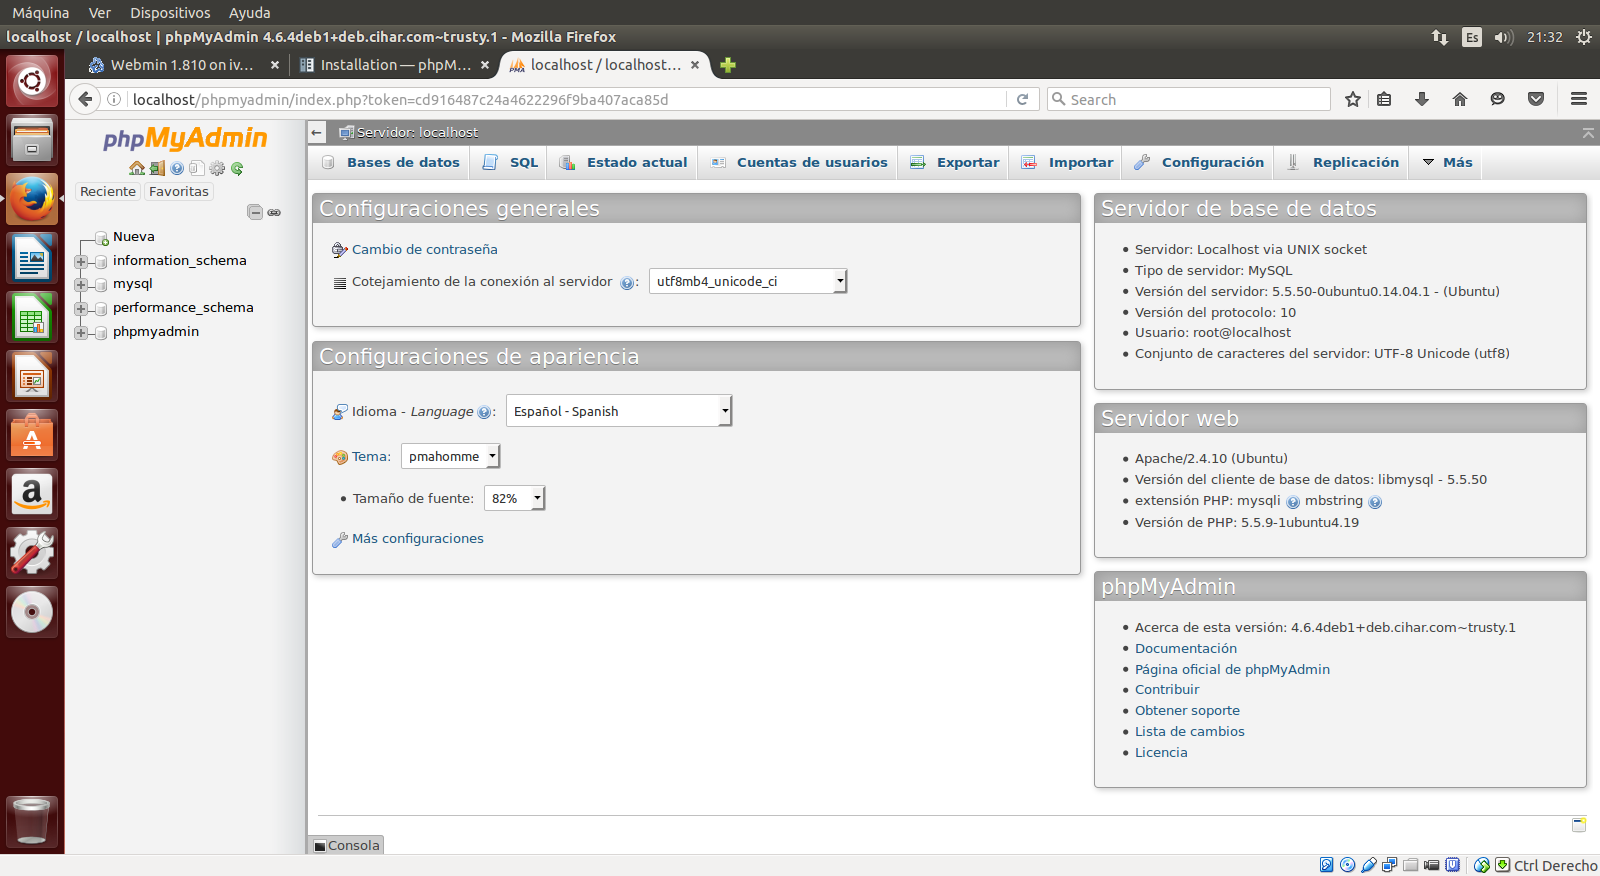
\includegraphics[width=0.7\linewidth]{PHpmyadminInicio}
		\caption[PHPmyadmin inicio]{Pantalla de inicio de phpmyadmin tras autenticarse como root.}
		\label{fig:PHpmyadminInicio}
	\end{figure}
	
	Si nos ponemos a fisgar en la herramienta, nos encontramos con la pestaña de base de datos:\\
	
	\begin{figure}[H]
		\centering
		\includegraphics[width=0.7\linewidth]{PHPMyadminDataBases}
		\caption[PHPmyadmin Data bases]{Bases de datos por defecto en phpmyadmin.}
		\label{fig:PHPMyadminDataBases}
	\end{figure}
	
	de las cuales se pueden ver estadísticas como la cantidad de datos que estas poseen, que como vemos, ninguna sobrepasa la cantidad por defecto. Esto nos lleva a la segunda parte de la pregunta:\\
	
	\textbf{¿Cómo modifico el tamaño máximo de base de datos que puedo administrar en phpmyadmin?}\\
	
	La primera respuesta que encontré estaba en stackoverflow, tras la cual busqué en php el parámetro que tenía que modificar(las páginas web consultadas están en \cite{phpMaxSize}). Según ambas respuestas, el parámetro que tengo que modificar se encuentra en el directorio $/etc/php/7.0/apache2/$ en el archivo \textbf{php.ini}. Tal parámetro es post\_max\_size, el cual define el tamaño máximo de datos permitido. También afecta a la subida de ficheros, lo que andábamos buscando. En principio, para terminar esta parte de la pregunta nos basta responder que con cambiar el valor de 8Mib a un valor mayor podremos subir bases de datos mayores. Sin embargo el parámetro también se puede cambiar a cero, lo que haría que se admitiese cualquier tamaño de base de datos para la subida.

	\begin{figure}[H]
		\centering
		\includegraphics[width=0.7\linewidth]{phpPostMaxSize}
		\caption[php post max size]{Modificación del parámetro post\_max\_size en el archivo php.ini.}
		\label{fig:phpPostMaxSize}
	\end{figure}
	
	Reiniciamos el servicio de apache2 y ya estará en funcionamiento.
	
\end{itemize}

\subsection{Otros servidores.}
	\begin{itemize}
		\item  \textbf{Visite al menos una de las webs de los software mencionados en la práctica y pruebe las demos que ofrecen realizando capturas de pantalla y comentando qué está	realizando.}\\
		
		Vamos a visitar la página web de DirectAdmin\cite{directadmin}, en la cual probaremos los servicios que ofrece como administrador web:\\
		
		\begin{figure}[H]
			\centering
			\includegraphics[width=0.7\linewidth]{directadminWeb}
			\caption[Web de DirectAdmin]{Página web de DirectAdmin}
			\caption{}
			\label{fig:directadminWeb}
		\end{figure}
		en la cual, podremos probar una demo de administrador:\\
		
		\begin{figure}[H]
			\centering
			\includegraphics[width=0.7\linewidth]{DirectAdminTryDemo}
			\caption[Try demo DirectAdmin]{Probar las demos. Login:demo\_admin,Password:demo}
			\label{fig:DirectAdminTryDemo}
		\end{figure}
		
		La página de inicio del servicio es la siguiente:\\
		
		\begin{figure}[H]
			\centering
			\includegraphics[width=0.7\linewidth]{DirectAdminStartPage}
			\caption[Pagina inicio direct admin]{Página de inicio de Directadmin como administrador.}
			\label{fig:DirectAdminStartPage}
		\end{figure}
		
		Vamos a ir mostrando distintas funcionalidades de la demo. Un ejemplo de ello es el monitor de servicios, desde el cual se pueden reiniciar o parar:\\
		
		\begin{figure}[H]
			\centering
			\includegraphics[width=0.7\linewidth]{DirectAdminServiceMonitor}
			\caption[Service monitor]{Monitor de servicios, localizado en herramientas de administrador(Admin Tool).}
			\label{fig:DirectAdminServiceMonitor}
		\end{figure}
		
		También nos encontramos con un editor de texto. En la web no podemos usarlo ya que está deshabilitado, pero con él podremos editar archivos sensibles para la configuración de nuestra página web, como sería httpd.conf:\\
		
		\begin{figure}[H]
			\centering
			\includegraphics[width=0.7\linewidth]{DirectAdminFileEditor}
			\caption[File Editor]{Editor de texto para modificar archivos sensibles de la configuración. No disponible en la demo.}
			\label{fig:DirectAdminFileEditor}
		\end{figure}
		
		También podemos crear cuantas de toda clase, como por ejemplo de administrador. Sin embargo, en la demo la creación está deshabilitada:\\
		
		\begin{figure}[H]
			\centering
			\includegraphics[width=0.7\linewidth]{DirectAdminCrearCuentaAdministrador}
			\caption[Cuenta Administrador]{Creación de la cuenta de administrador, con login ivan y cuenta de correo fake@fakemail.com. Se encuentra en Server Management.}
			\label{fig:DirectAdminCrearCuentaAdministrador}
		\end{figure}
		
		Por último, en la sección Extra Features, nos podemos encontrar con los datos de las actividades periódicas programadas con cron de todos los usuarios:\\
		
		\begin{figure}[H]
			\centering
			\includegraphics[width=0.7\linewidth]{DirectAdminCronJobs}
			\caption[CronJobs]{Trabajos periódicos programados por cron de todos los usuarios.}
			\label{fig:DirectAdminCronJobs}
		\end{figure}

	\end{itemize}
	
\section{Automatización de tareas.}

En esta sección se aborda la creación de scripts, el uso de la shell y algunos comandos útiles para la automatización de tareas. Un ejemplo de comandos son $grep$\cite{man_grep}, $find$\cite{man_find}, $awk$\cite{man_awk} y $sed$\cite{man_sed}.

\begin{itemize}
	\item  \textbf{Ejecute los ejemplos de find, grep y escriba el script que haga uso de sed para cambiar la configuración de ssh y reiniciar el servicio.}\\
	
	Ejecución del ejemplo de find:\\
	
	\begin{figure}[H]
		\centering
		\includegraphics[width=0.7\linewidth]{ejemploFind}
		\caption[Ejemplo find]{Ejecución del ejemplo de Find, en donde se recopilan los Pdfs dentro del directorio Documentos en el directorio PDFs}
		\label{fig:ejemploFind}
	\end{figure}
	
	\begin{figure}[H]
		\centering
		\includegraphics[width=0.7\linewidth]{PDFsGuardados}
		\caption[PDFs almacenados.]{Directorio PDFs tras la ejecución de find.}
		\label{fig:PDFsGuardados}
	\end{figure}
	
	Ejecución del ejemplo de grep:\\
	
	\begin{figure}[H]
		\centering
		\includegraphics[width=0.7\linewidth]{EjemploGrep}
		\caption[Ejemplo grep]{Ejecución del ejemplo de grep. En el se busca la información de los precesos que tengan que ver con firefox.}
		\label{fig:EjemploGrep}
	\end{figure}
	
	El script que usaremos será el siguiente, que deberá ser ejecutado como administrador:\\
	
	
	cp /etc/ssh/ssh\_config /etc/ssh/ssh\_config.original\\
	sed 's/\#   ForwardX11 no/   ForwardX11 no/g' /etc/ssh/ssh\_config\\
	service ssh restart\\
	
	
	En el, primero copiamos la configuración original por si acaso en un archivo aparte. Luego, en la segunda linea, se sustituye la linea comentada en la que se invalida la posibilidad de poder usar interfaz gráfica en conexiones ssh por la misma linea descomentada. En la última linea se reinicia el servicio. Aquí está la ejecución del script:\\
	
	\begin{figure}[H]
		\centering
		\includegraphics[width=0.7\linewidth]{SalidaScript}
		\caption[Salida script]{Salida producida por el script. En el se ve que se modifica la linea deseada.}
		\label{fig:SalidaScript}
	\end{figure}
	
	\item \textbf{Escriba el script para cambiar el acceso a ssh usando PHP o Python.}
	
	Yo he escogido python.???

	\item \textbf{Windows Powershell.} Abra una consola de Powershell y pruebe a parar un programa en ejecución (p.ej), realice capturas de pantalla y comente lo que muestra.\\
	
	Para averiguar que comando es el necesario para parar un proceso, escribimos en la powershell el comando Get-Command -verb stop:\\
	
	\begin{figure}[H]
		\centering
		\includegraphics[width=0.7\linewidth]{PoweshellGetCommand}
		\caption[Powershell]{Comando get-command de la powershell para encontrar el comando que para un programa.}
		\label{fig:PoweshellGetCommand}
	\end{figure}

	que como sospechábamos, era Stop-Process. Ahora probamos a obtener los procesos activos y vamos a eliminar el nuestro:\\
	
	\begin{figure}[H]
		\centering
		\includegraphics[width=0.7\linewidth]{PowershellProcesos}
		\caption[Procesos powershell]{Información de los precesos que lleva a cabo windows. Información suministrada por el comando Get-Process de PowerShell. ID del proceso encargado del Server Manager:1560.}
		\label{fig:PowershellProcesos}
	\end{figure}
	
	Puesto que estamos ejecutando el Server Manager, con Pid 1560, para pararlo tenemos que usar el comando antes buscado: stop-process 1560, tras lo cual, paramos el proceso:\\
	
	\begin{figure}[H]
		\centering
		\includegraphics[width=0.7\linewidth]{Powershellstopprocess}
		\caption[Powershell stop process]{Comando stop-process de la powershell sobre el server manager de windows. Tras esto, hemos vuelto a usar get-process.}
		\label{fig:Powershellstopprocess}
	\end{figure}
	
	Como vemos en la ventana, hemos parado el proceso y no vemos rastro de la ventana ni del nombre del proceso entre los procesos que lista get-process.


\end{itemize}





\newpage
\begin{thebibliography}{xxx}
	\bibitem{yum} http://linux.die.net/man/8/yum
	\bibitem{yum.conf} http://linux.die.net/man/5/yum.conf
	\bibitem{apt} http://linux.die.net/man/8/apt
	\bibitem{apt.conf} http://linux.die.net/man/5/apt.conf
	\bibitem{yast} https://es.opensuse.org
	\bibitem{telnet} http://linux.die.net/man/1/telnet
	\bibitem{ssh} http://linux.die.net/man/1/ssh
	\bibitem{ssh-client} http://linux.die.net/man/1/ssh
	\bibitem{ssh-keygen} http://linux.die.net/man/1/ssh-keygen
	\bibitem{copy-id} http://linux.die.net/man/1/ssh-copy-id
	\bibitem{sshd} http://www.freebsd.org/cgi/man.cgi?sshd(8)
	\bibitem{sshd_config} https://www.freebsd.org/cgi/man.cgi?sshd\_config(5)
	\bibitem{terminator} http://manpages.ubuntu.com/manpages/precise/man1/terminator.1.html
	\bibitem{screen} https://www.gnu.org/software/screen/manual/screen.html
	\bibitem{fail2ban} http://www.fail2ban.org/wiki/index.php/MANUAL\_0\_8
	\bibitem{w3tech} https://w3techs.com
	\bibitem{liteSpeed} https://www.litespeedtech.com/products/litespeed-web-server/overview
	\bibitem{Tomcat} http://tomcat.apache.org/
	\bibitem{nodejs} https://nodejs.org/en/
	\bibitem{tutorialFTP} https://technet.microsoft.com/es-es/library/hh831655(v=ws.11).aspx\#Step2
	\bibitem{patch} http://fedoraproject.org/wiki/VMWare
	\bibitem{diff} http://man7.org/linux/man-pages/man1/diff.1.html
	\bibitem{webadinInstalation} http://www.webmin.com/deb.html
	\bibitem{phpMyAdmin} https://docs.phpmyadmin.net
	\bibitem{phpMaxSize} http://php.net/manual/es/ini.core.php\#ini.post-max-size\\
	http://stackoverflow.com/questions/3958615/import-file-size-limit-in-phpmyadmin
	\bibitem{directadmin} https://www.directadmin.com/
	\bibitem{man_grep} https://www.gnu.org/software/grep/manual/grep.html
	\bibitem{man_find} http://man7.org/linux/man-pages/man1/find.1.html
	\bibitem{man_awk} https://www.gnu.org/software/gawk/manual/gawk.html\#Running-gawk
	\bibitem{man_sed} http://linux.die.net/man/1/sed
	
	
\end{thebibliography}
\end{document}